% \LaTeX-Main\
%% The LaTeX package tcolorbox - version 5.1.1 (2022/06/24)
%% tcolorbox-tutorial-poster.tex: a tutorial for poster creation with tcolorbox
%%
%% -------------------------------------------------------------------------------------------
%% Copyright (c) 2006-2022 by Prof. Dr. Dr. Thomas F. Sturm <thomas dot sturm at unibw dot de>
%% -------------------------------------------------------------------------------------------
%%
%% This work may be distributed and/or modified under the
%% conditions of the LaTeX Project Public License, either version 1.3
%% of this license or (at your option) any later version.
%% The latest version of this license is in
%%   http://www.latex-project.org/lppl.txt
%% and version 1.3 or later is part of all distributions of LaTeX
%% version 2005/12/01 or later.
%%
%% This work has the LPPL maintenance status `author-maintained'.
%%
%% This work consists of all files listed in README
%%
% arara: pdflatex: { shell: yes }
% arara: pdflatex: { shell: yes }
\documentclass[36pt]{article}

%\usepackage[a0paper,landscape]{geometry}
\usepackage[paperwidth=180cm,paperheight=120cm]{geometry}
\usepackage{layout}
\usepackage{lipsum}
\usepackage{lmodern}
\usepackage{enumerate}
\usepackage[poster]{tcolorbox}
\usepackage[round]{natbib}
\renewcommand{\bibsection}{} % works with natbib get rid of the Reference in the bibliography (We already have it in the title of the box
\tcbuselibrary{minted} % <- replace by \tcbuselibrary{listings}, if minted does not work for you

\pagestyle{empty}

\tcbset{
  mylisting/.style={enhanced jigsaw,size=minimal,toprule=0.5mm,bottomrule=0.5mm,boxsep=2mm,oversize,
  colback=white,opacityback=0.75,listing only}
}

\newtcblisting{guidelisting}[1]{mylisting,#1}
\begin{document}
\begin{tcbposter}[
  coverage = {
      spread,
      interior style={top color=white,bottom color=white!50!red},
      watermark text={Cornell Poster},
      watermark color=white,
  },
  poster   = {showframe,columns=4,rows=5},
  fontsize = 36pt,
  boxes = {
    enhanced standard jigsaw,sharp corners=downhill,arc=3mm,boxrule=1mm,
    colback=white,opacityback=0.75,colframe=blue,
    title style={left color=black,right color=cyan},
    fonttitle=\bfseries\Large\scshape,
    left=2cm,
    right=2cm
  },
]

%----
\posterbox[blankest,interior engine=path,height=9cm,
halign=center,valign=center,fontupper=\bfseries\large,colupper=red!25!black,
underlay={
\node[right,inner sep=0pt,outer sep=0pt] at (frame.west) {\includegraphics[height=9cm]{pink_marble.png}};
\node[left,inner sep=0pt,outer sep=0pt] at (frame.east) {\includegraphics[height=9cm]{crinklepaper.png}};
},
]{
name=title,
column=1,
span=4,
below=top}{
\resizebox{72cm}{!}
{ \bfseries\Huge Reproducible Transparent Carboncycle Models }\\[3mm]
{ \bfseries\Large An Open Source Biogeochemical Model Database}\\[2mm]
Hans.Mustermann@deepthought.university
}


\posterbox[adjusted title=Easy Model Creation And Inspection]{
  name=overview,
  column=1,
  below=title,
  %rowspan=2,
  %below=title,
  }{
	\begin{enumerate}
	\item
	bgc\_md2 is an open source python package availabe on GitHub, developed at the Max-Planck-Institut for BioGeoChemistry in Jena and more recently  in Yiqi Luo's Ecolab at NAU in Flagstaff and Cornell in Ithaca
	\item
	A set of libraries that can be used in other python scripts or interactively (jupyter or IPython )
	The picture shows a jupiter widget showing a table of models. The orange buttons can be clicked to 
	expand or collape a more detailed view of the particular model.
	\item
	$>$ 30 published vegetation, soil or ecosystems models in a format that
	for symbolic and numeric computations
	\item
	A set of special datatypes that describe components of the models and functions that operate on these datatypes
	\item 
	A userinterface that uses a graph library to compute what is computable and can be used for comparisons.
	\end{enumerate}

\section*{Inspection from different angels}
\subsection*{Analysis with symbolic tools}
	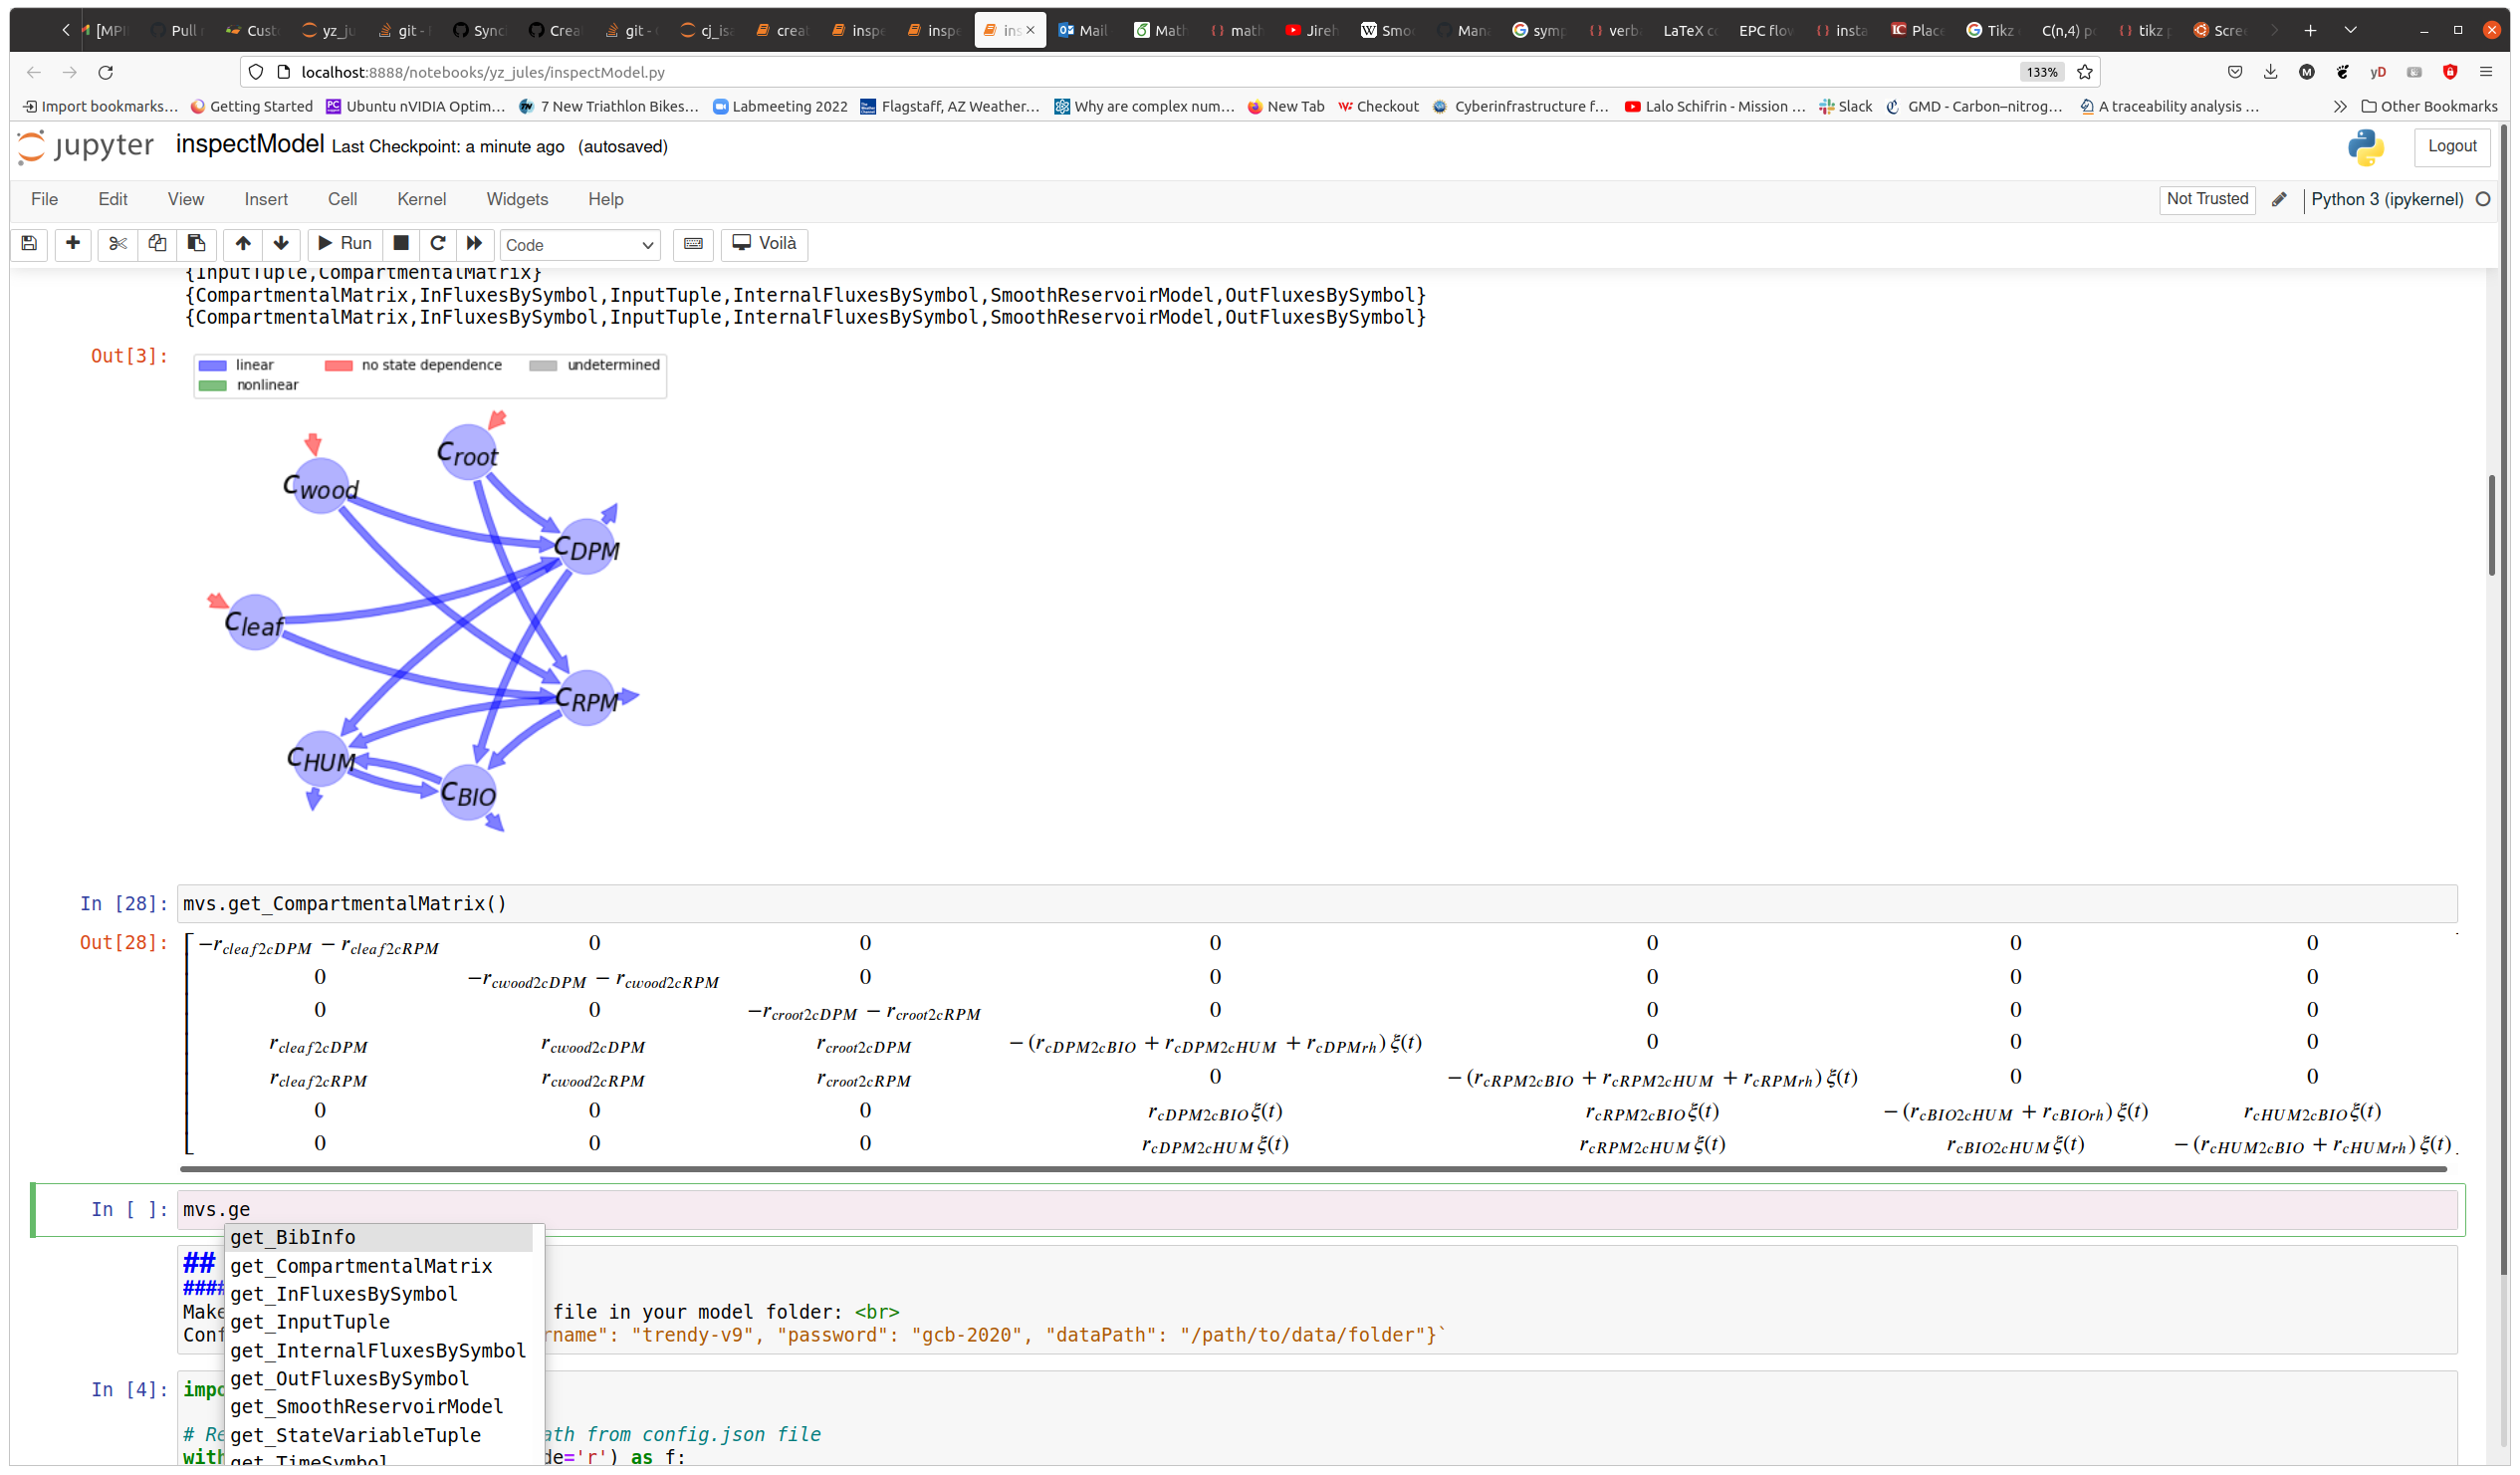
\includegraphics[width=\columnwidth]{mvsTabScreen.png}
	\begin{enumerate}
	\item 
	the structure (graph both in the mathematical and visual sense) can be derived from the symbolic description
	\item other properties are flux equations the compartmental matrix
	\end{enumerate}
	{\bfseries\large or numerically \dots}\\
	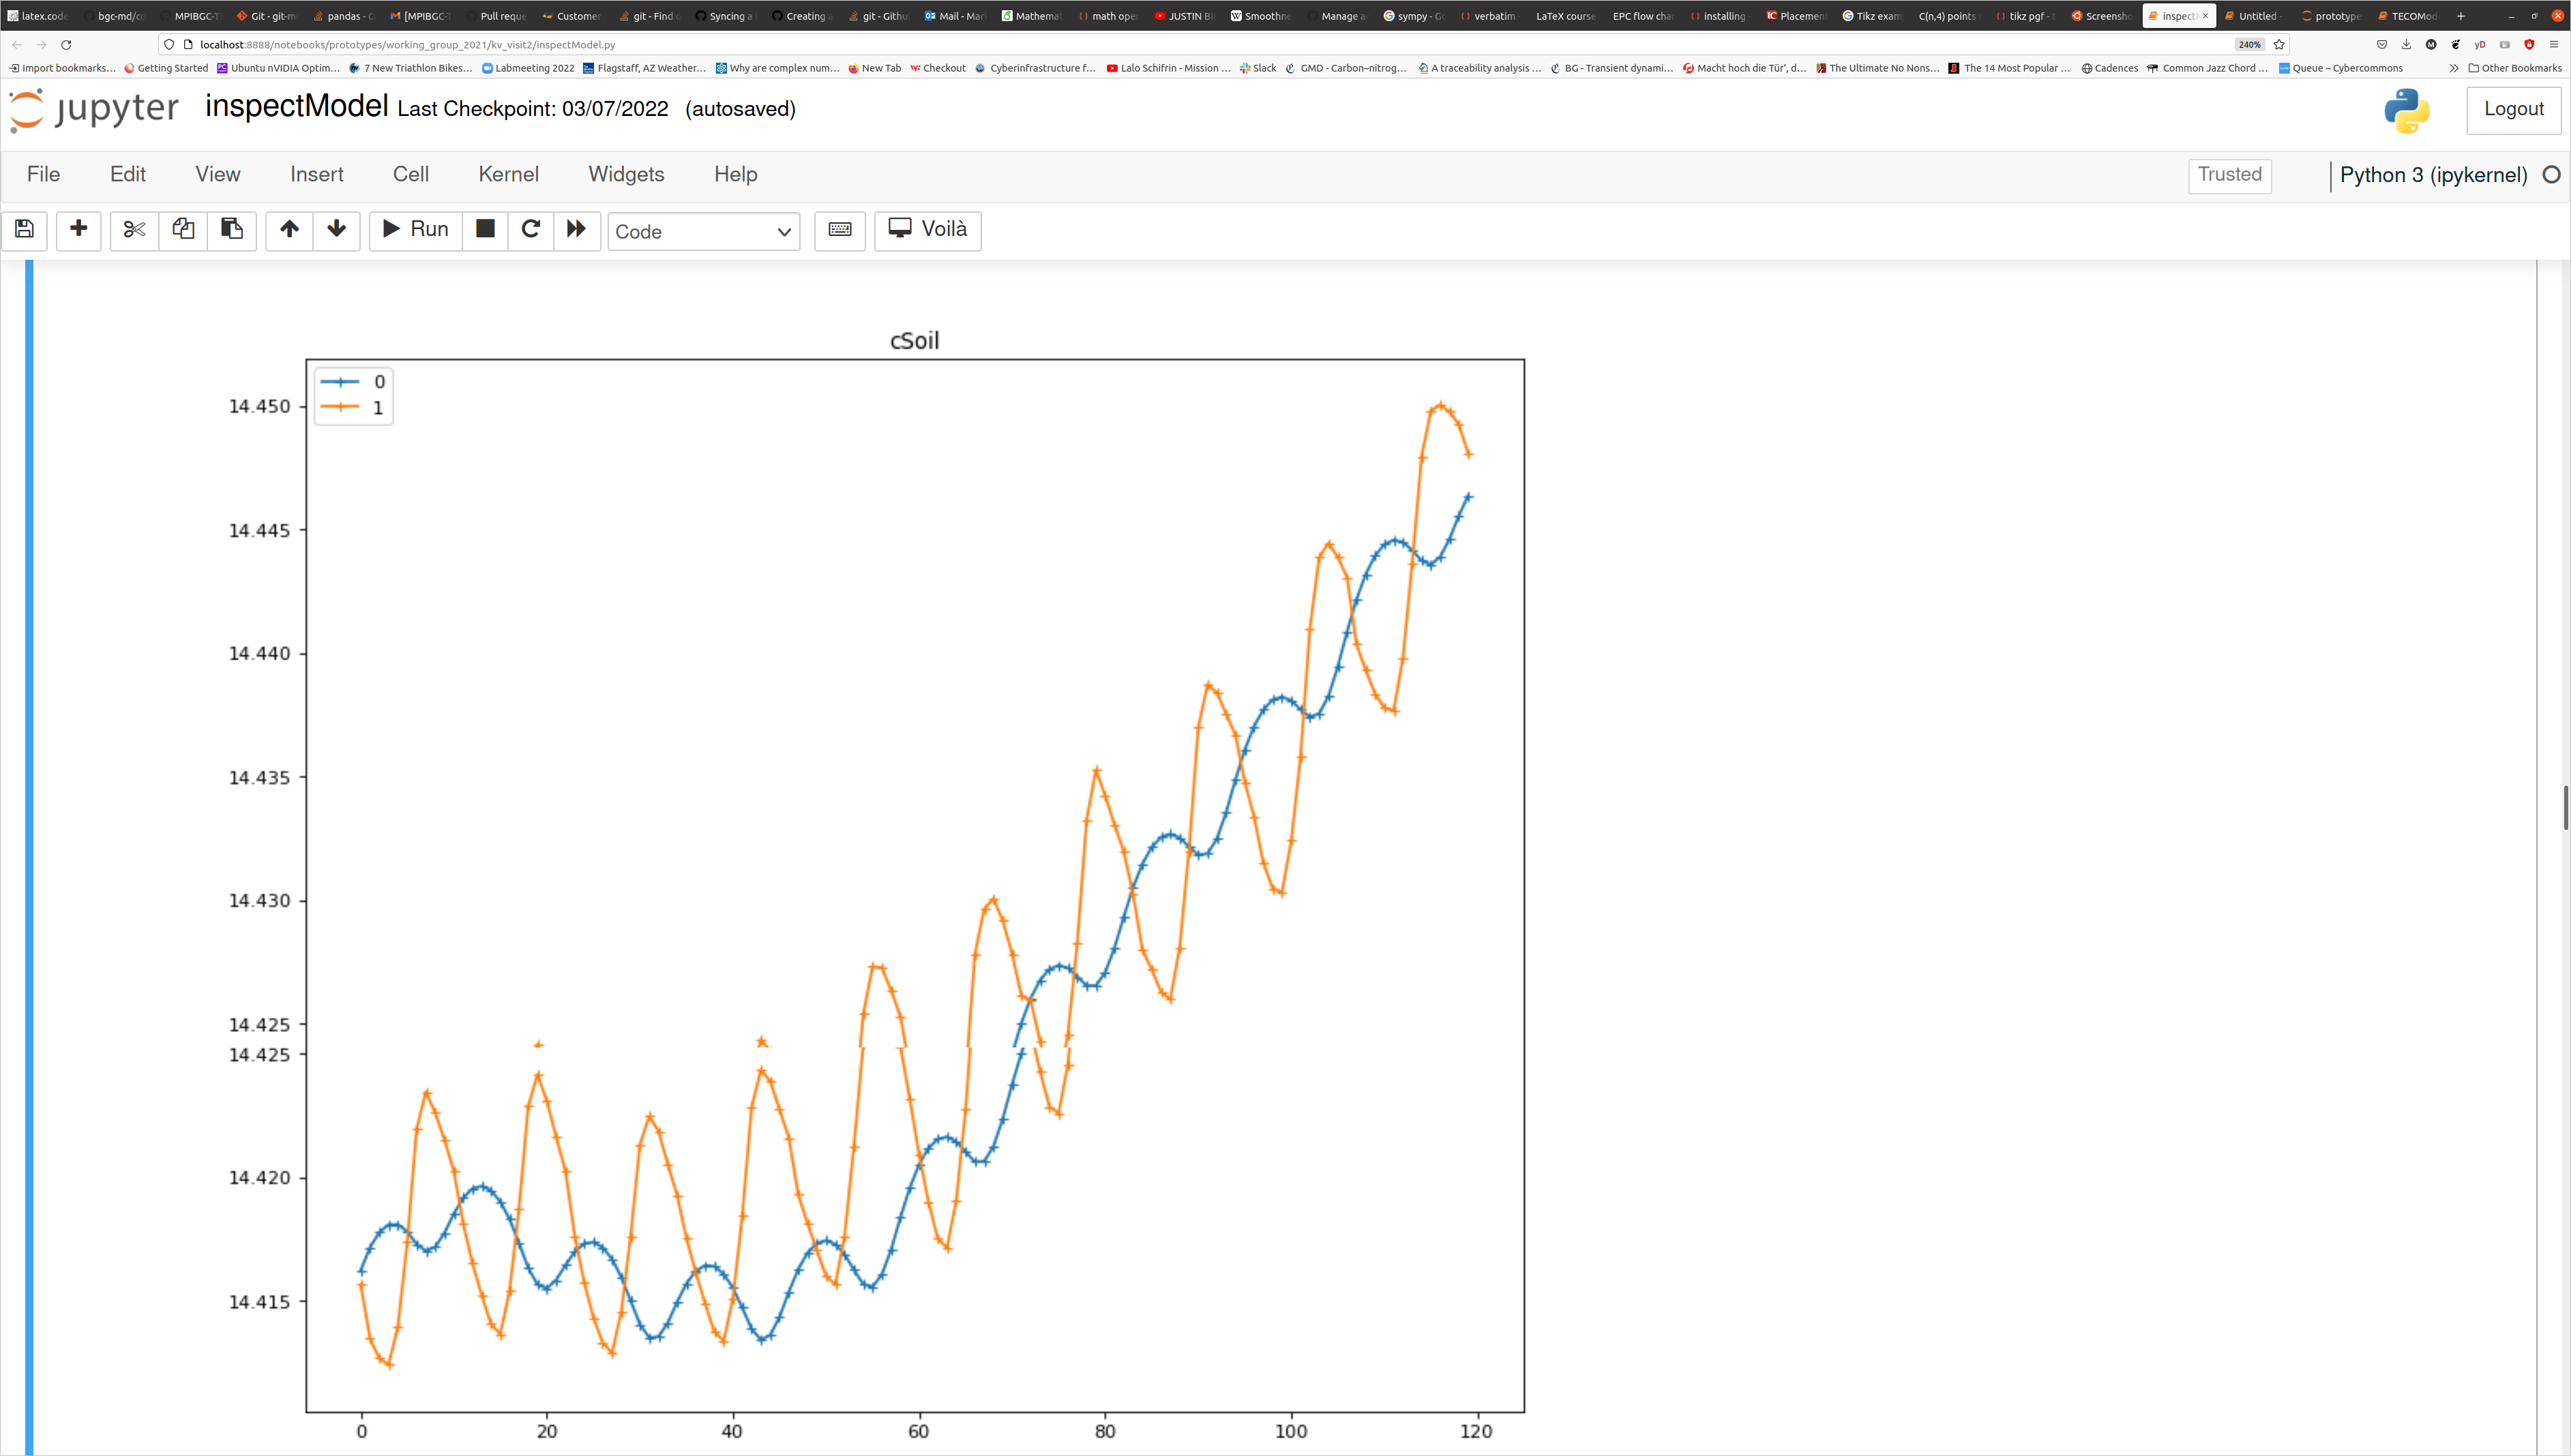
\includegraphics[width=.5\columnwidth]{DataAssimilation.png}
	\begin{enumerate}
	\item 
	the symbolic model description can be parameterized and transformed into a numeric model
	\item The picture shows the data assimilation result for the above model using trendy data.
	\end{enumerate}
}

%%%%%%%%%%%%%%%%%%%%%%%%%%%%%%%%%%%%%%%%%%%%%%%%%%%%%%%%%%%%%%%%%%%%%%%%%%%%%%%%%%%%%----
\posterbox[adjusted title=Comparability w.r.t. Common Diagnostics]{
  name=ModelIntercomparison,
  column=2,
  span=2,
  below=title,
  %rowspan=2,
  %sequence=1 between overview and bottom then 2 between title and bottom
  }{
	%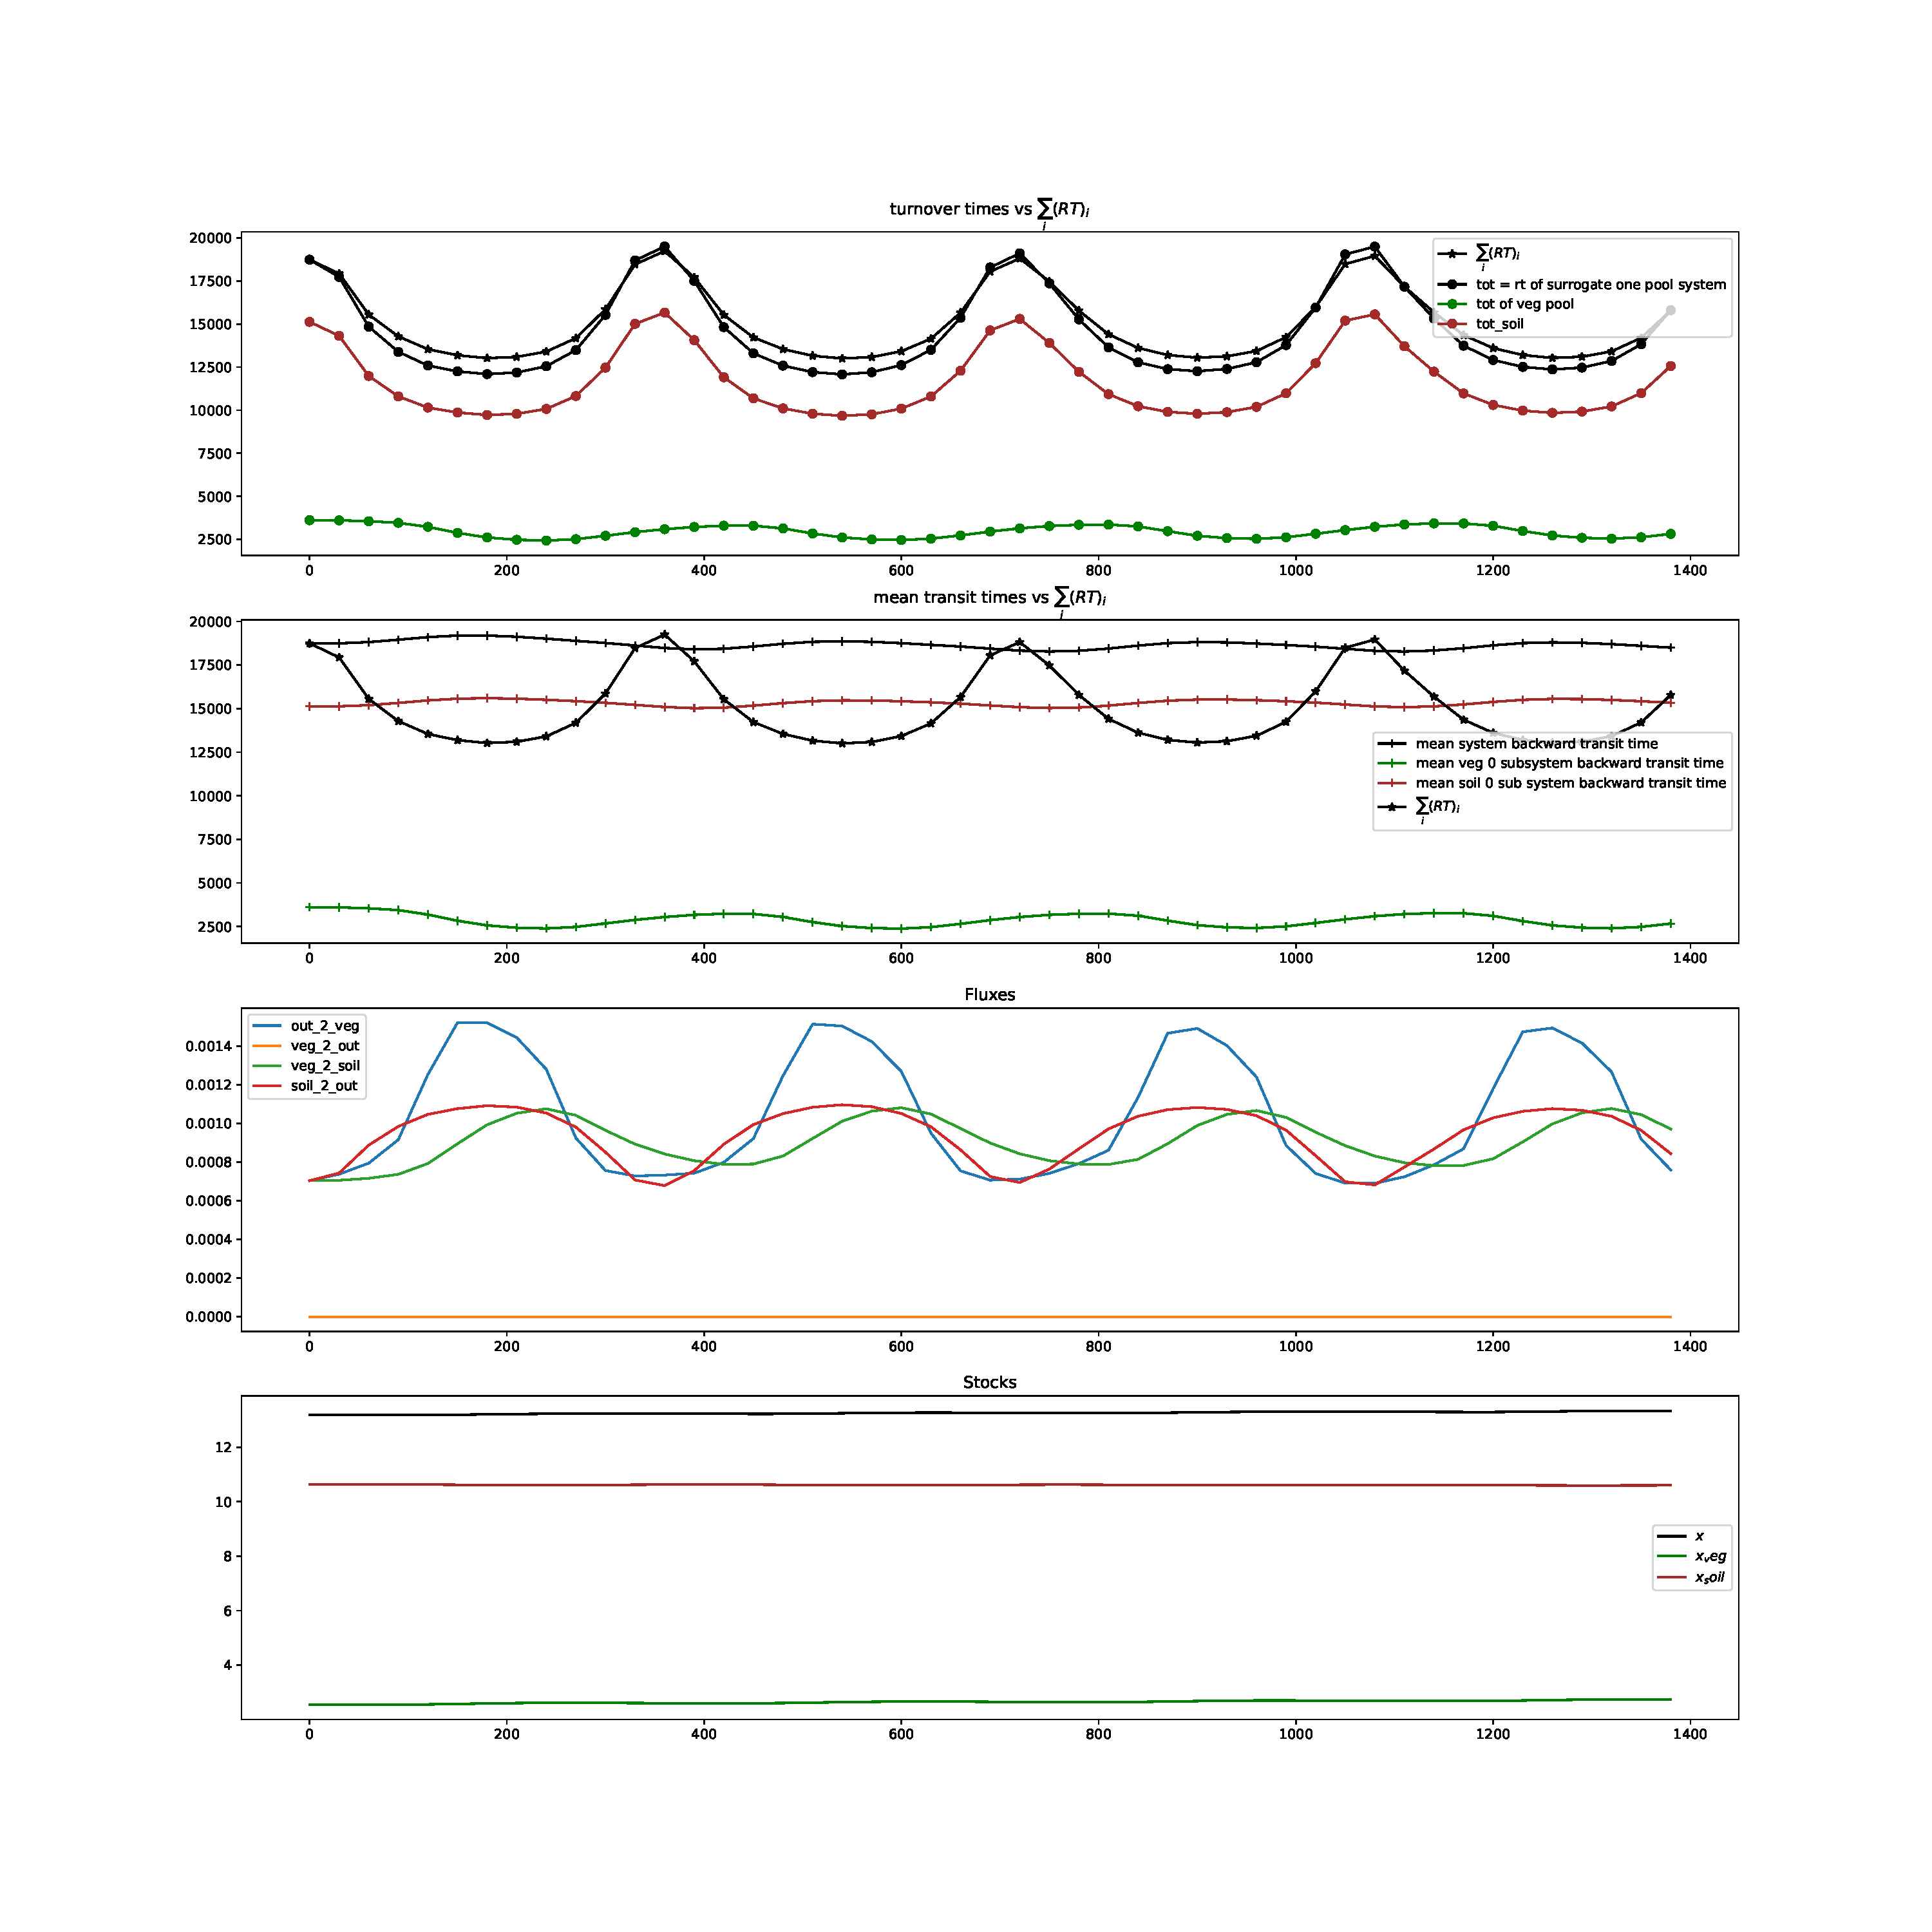
\includegraphics[width=\columnwidth]{system.pdf}

\begin{center}
	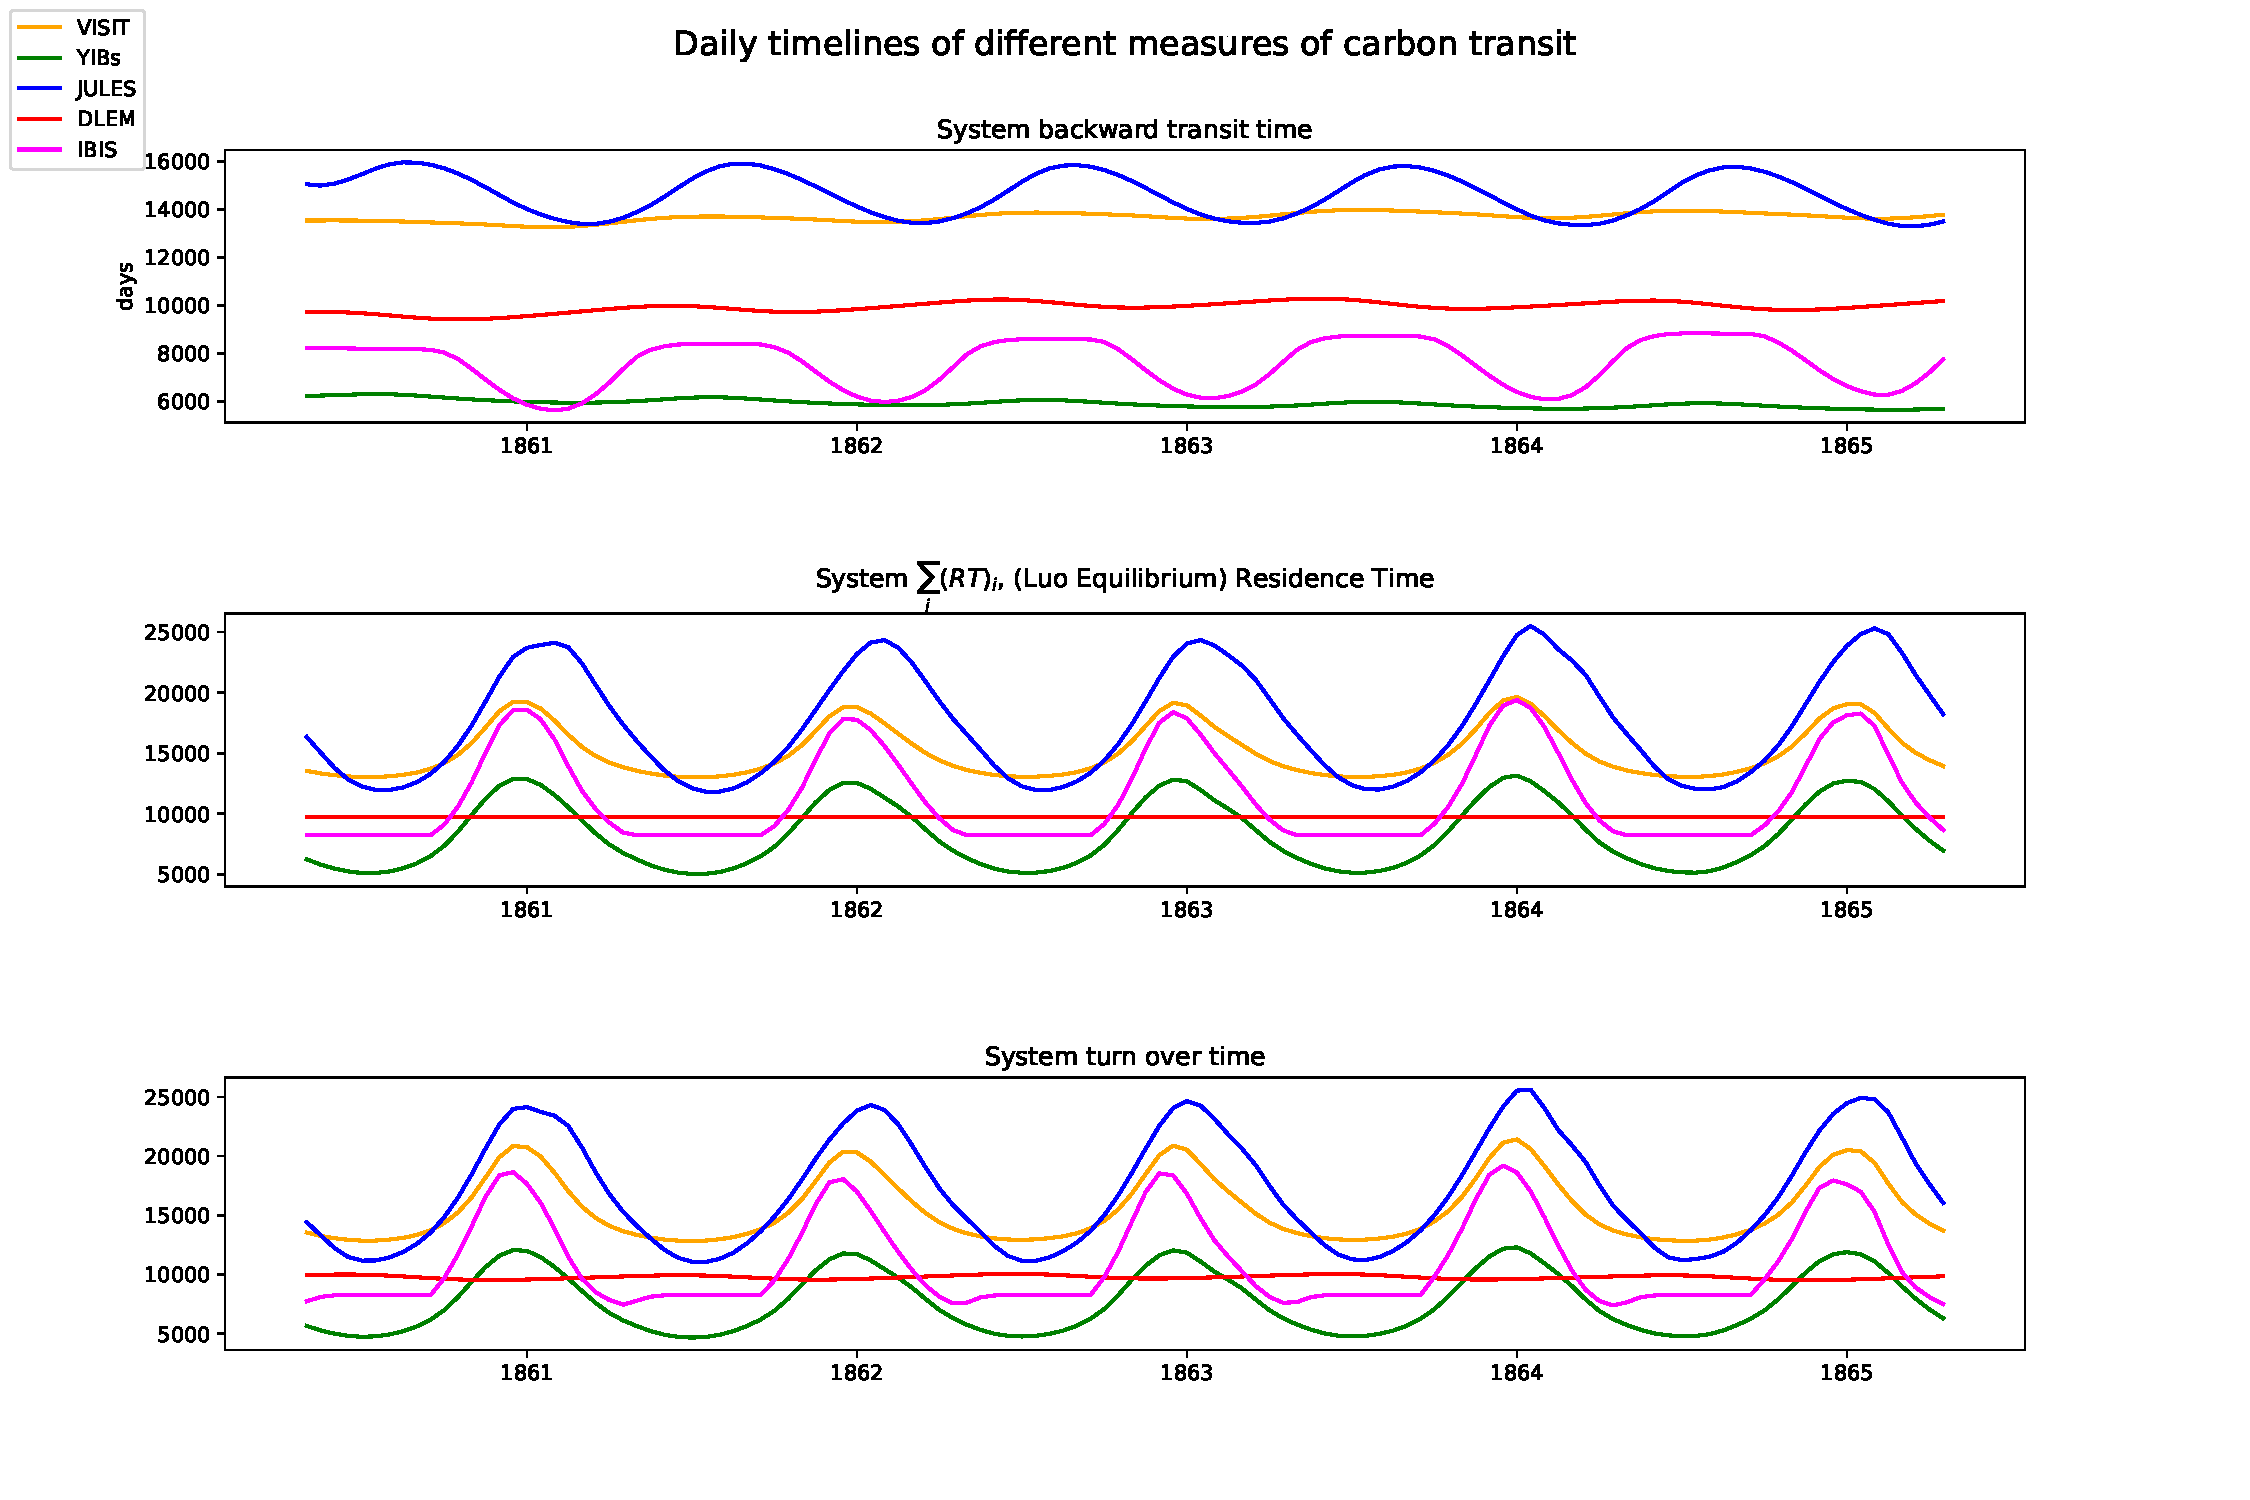
\includegraphics[width=.245\columnwidth]{test.pdf}
	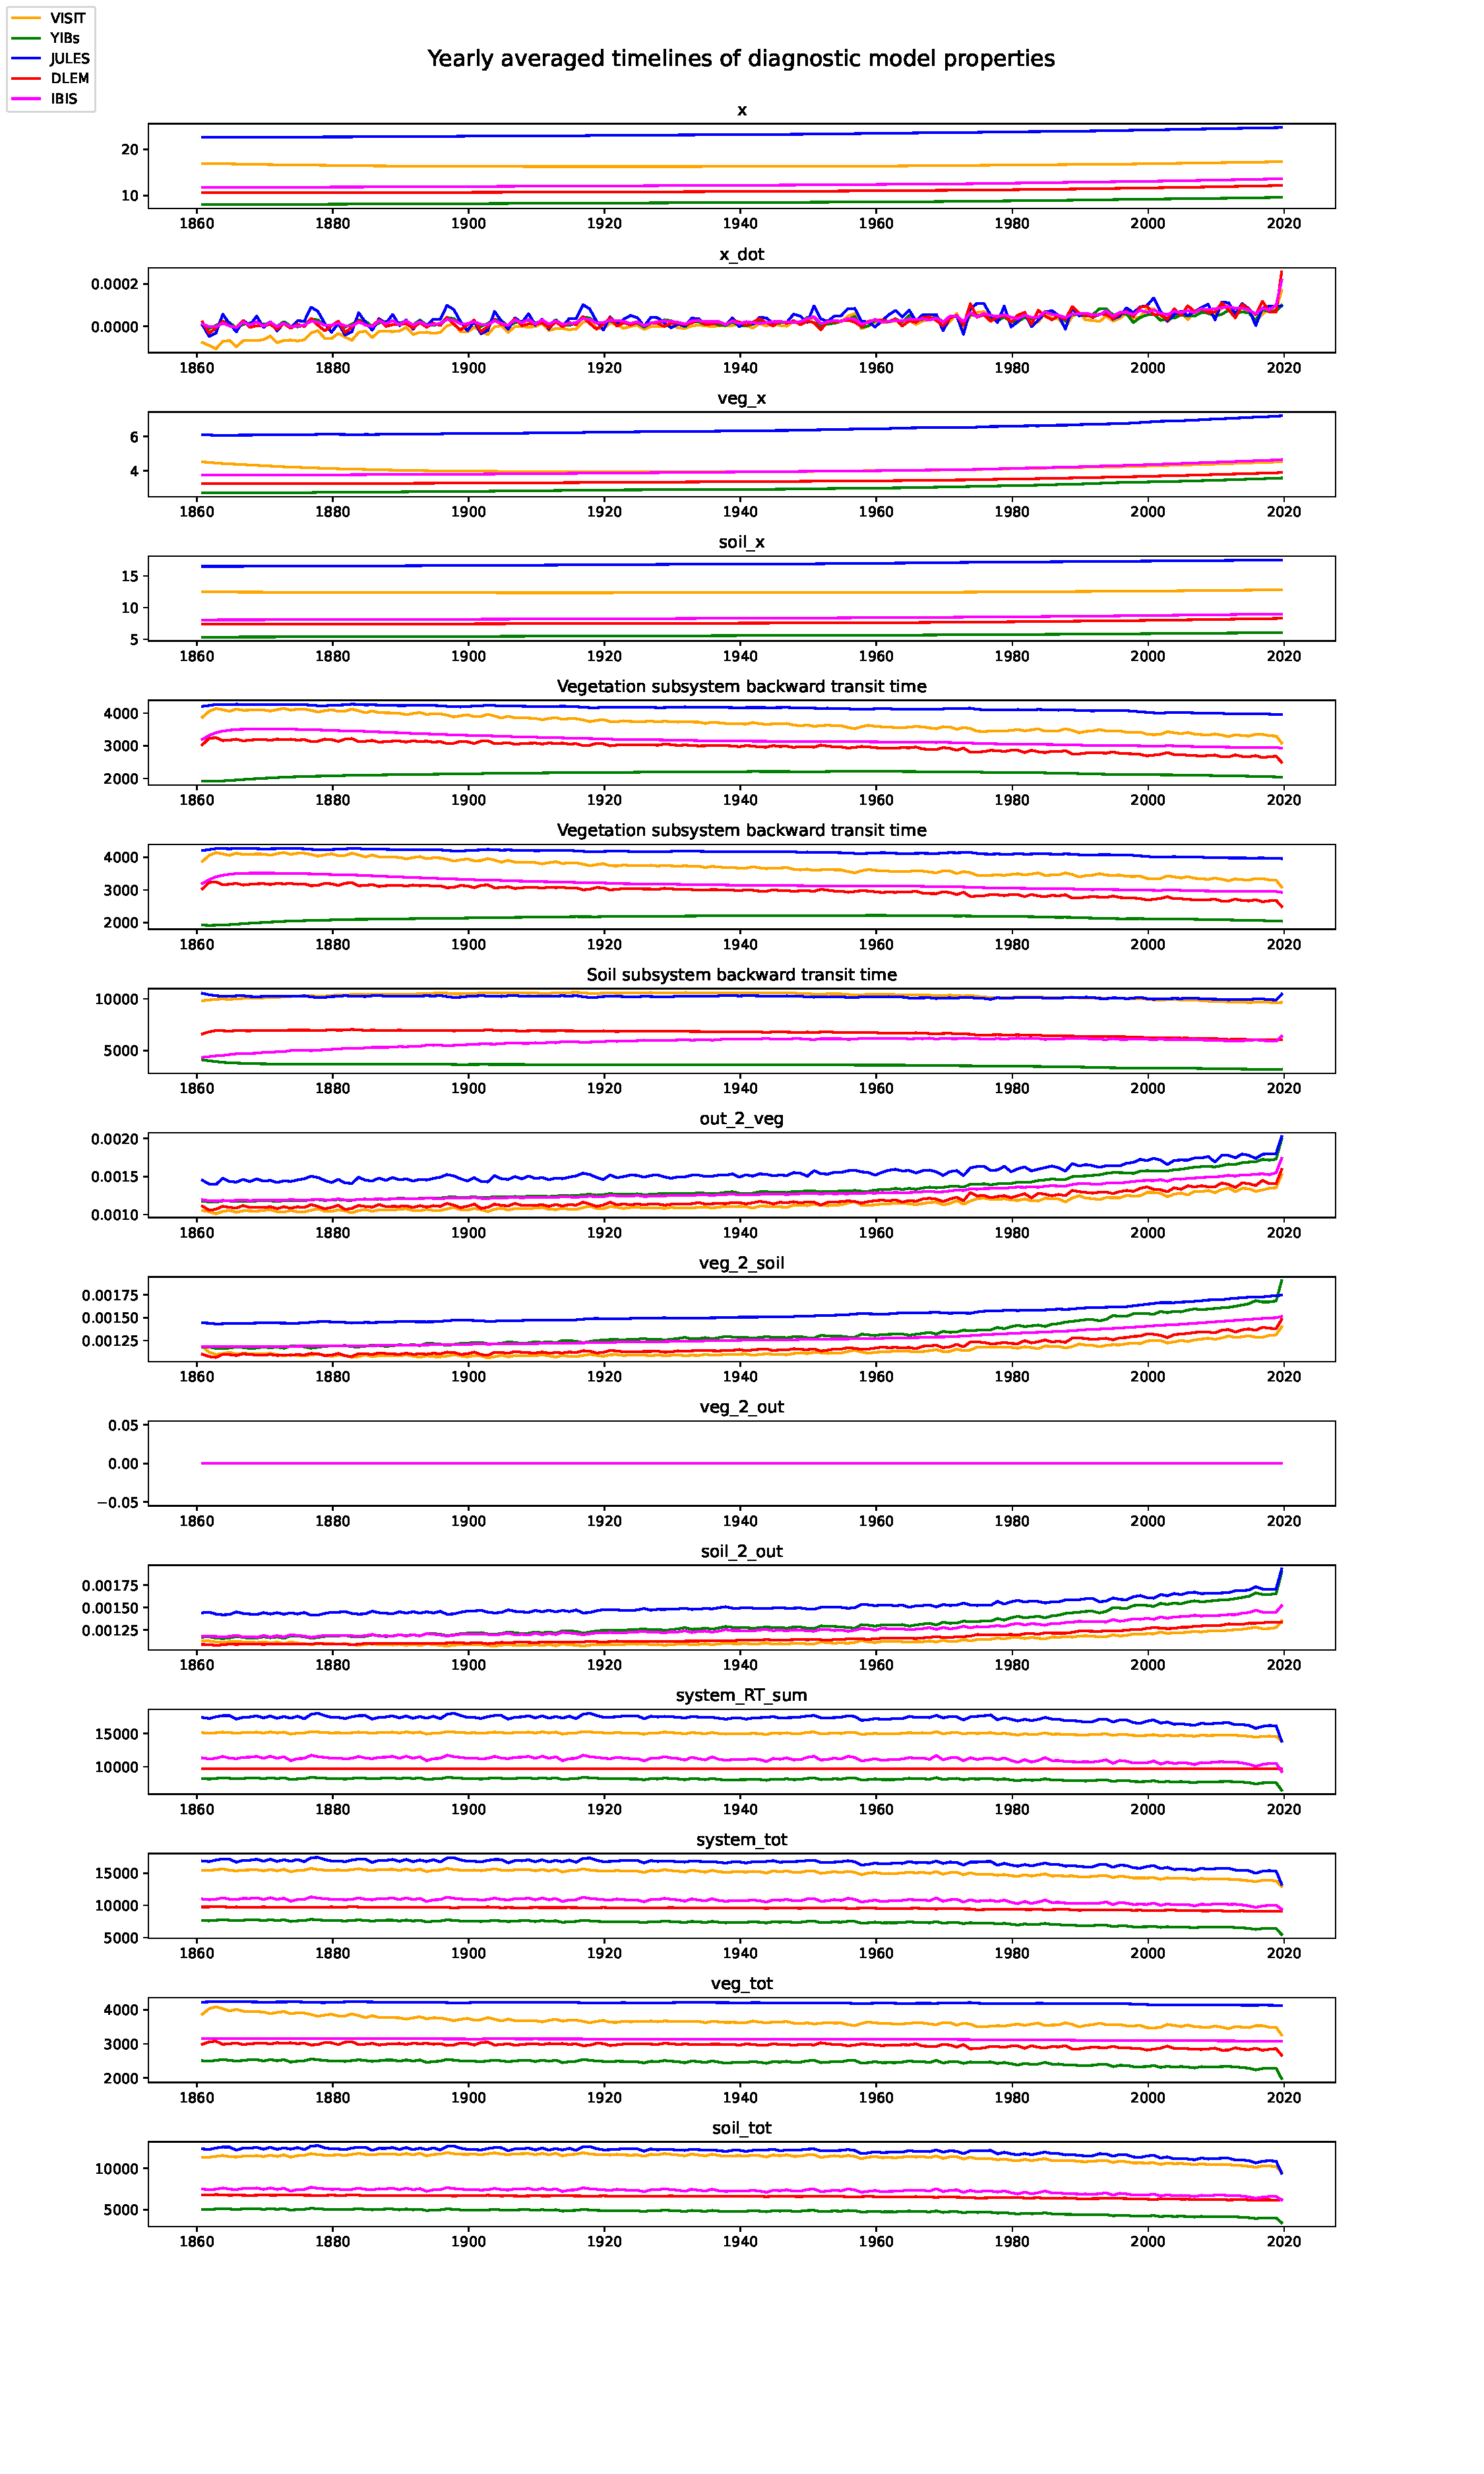
\includegraphics[width=.245\columnwidth]{test_yearly.pdf}
	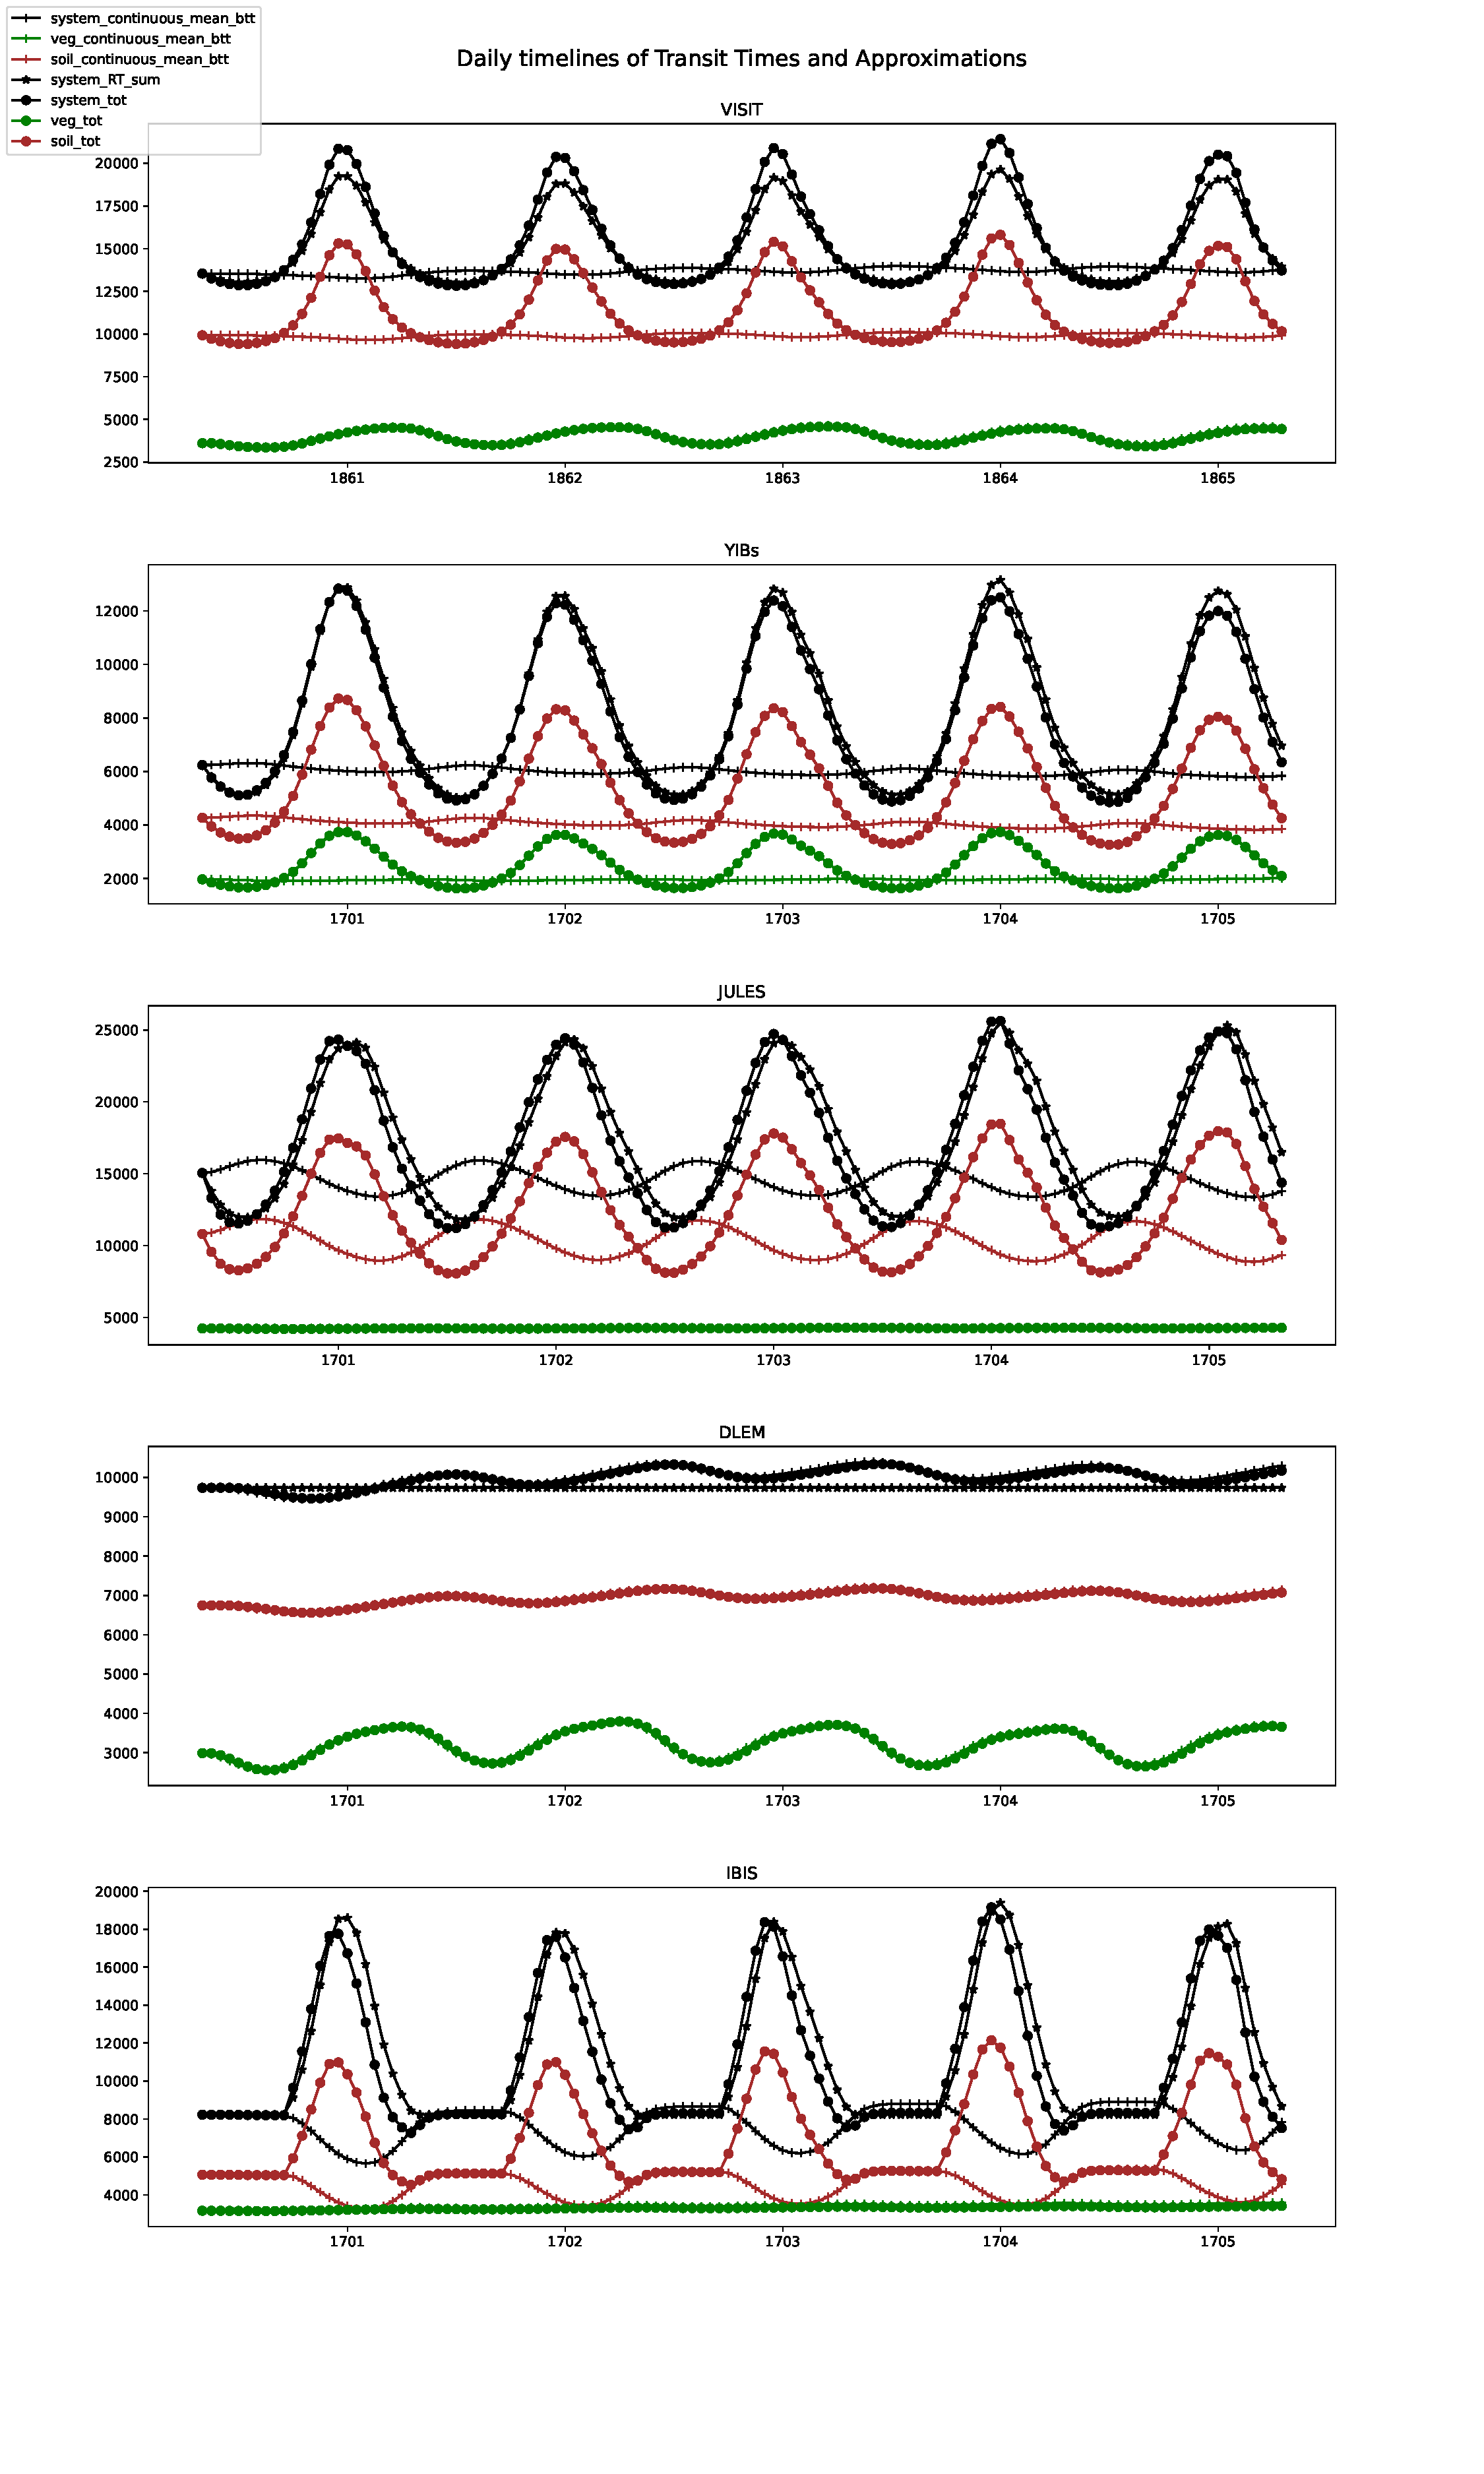
\includegraphics[width=.245\columnwidth]{test2_fine.pdf}
	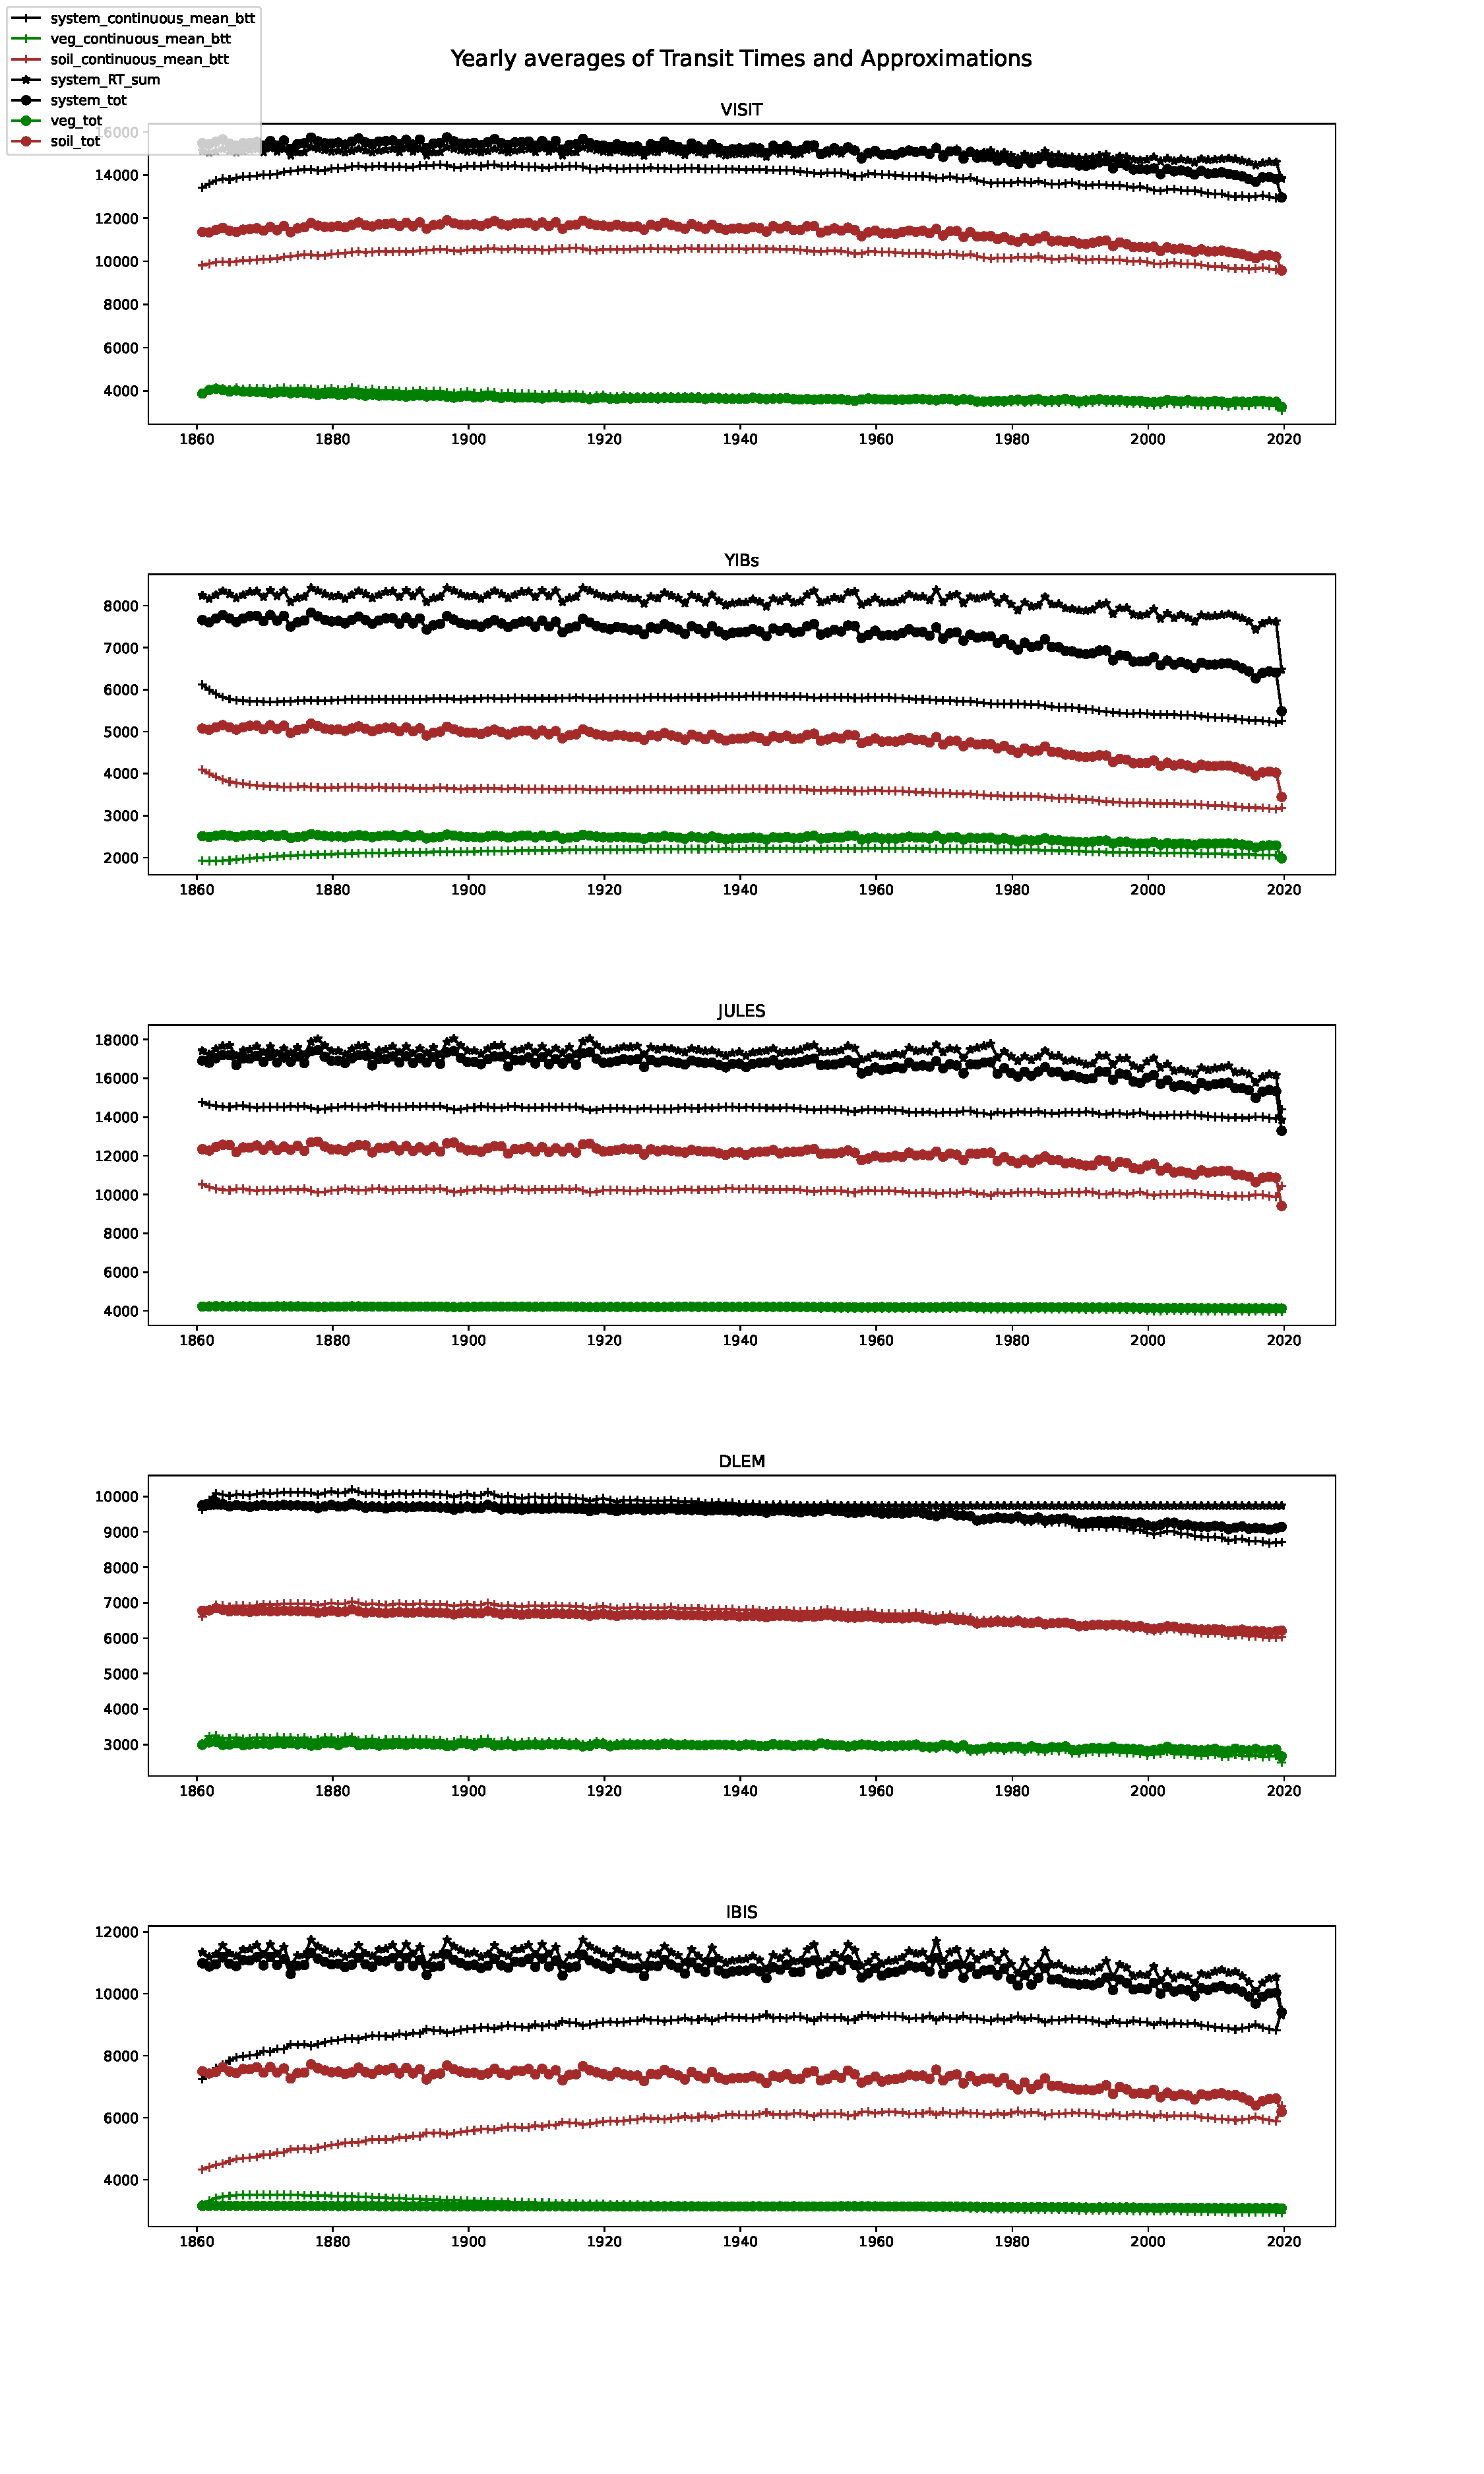
\includegraphics[width=.245\columnwidth]{test2_yearly.pdf}
	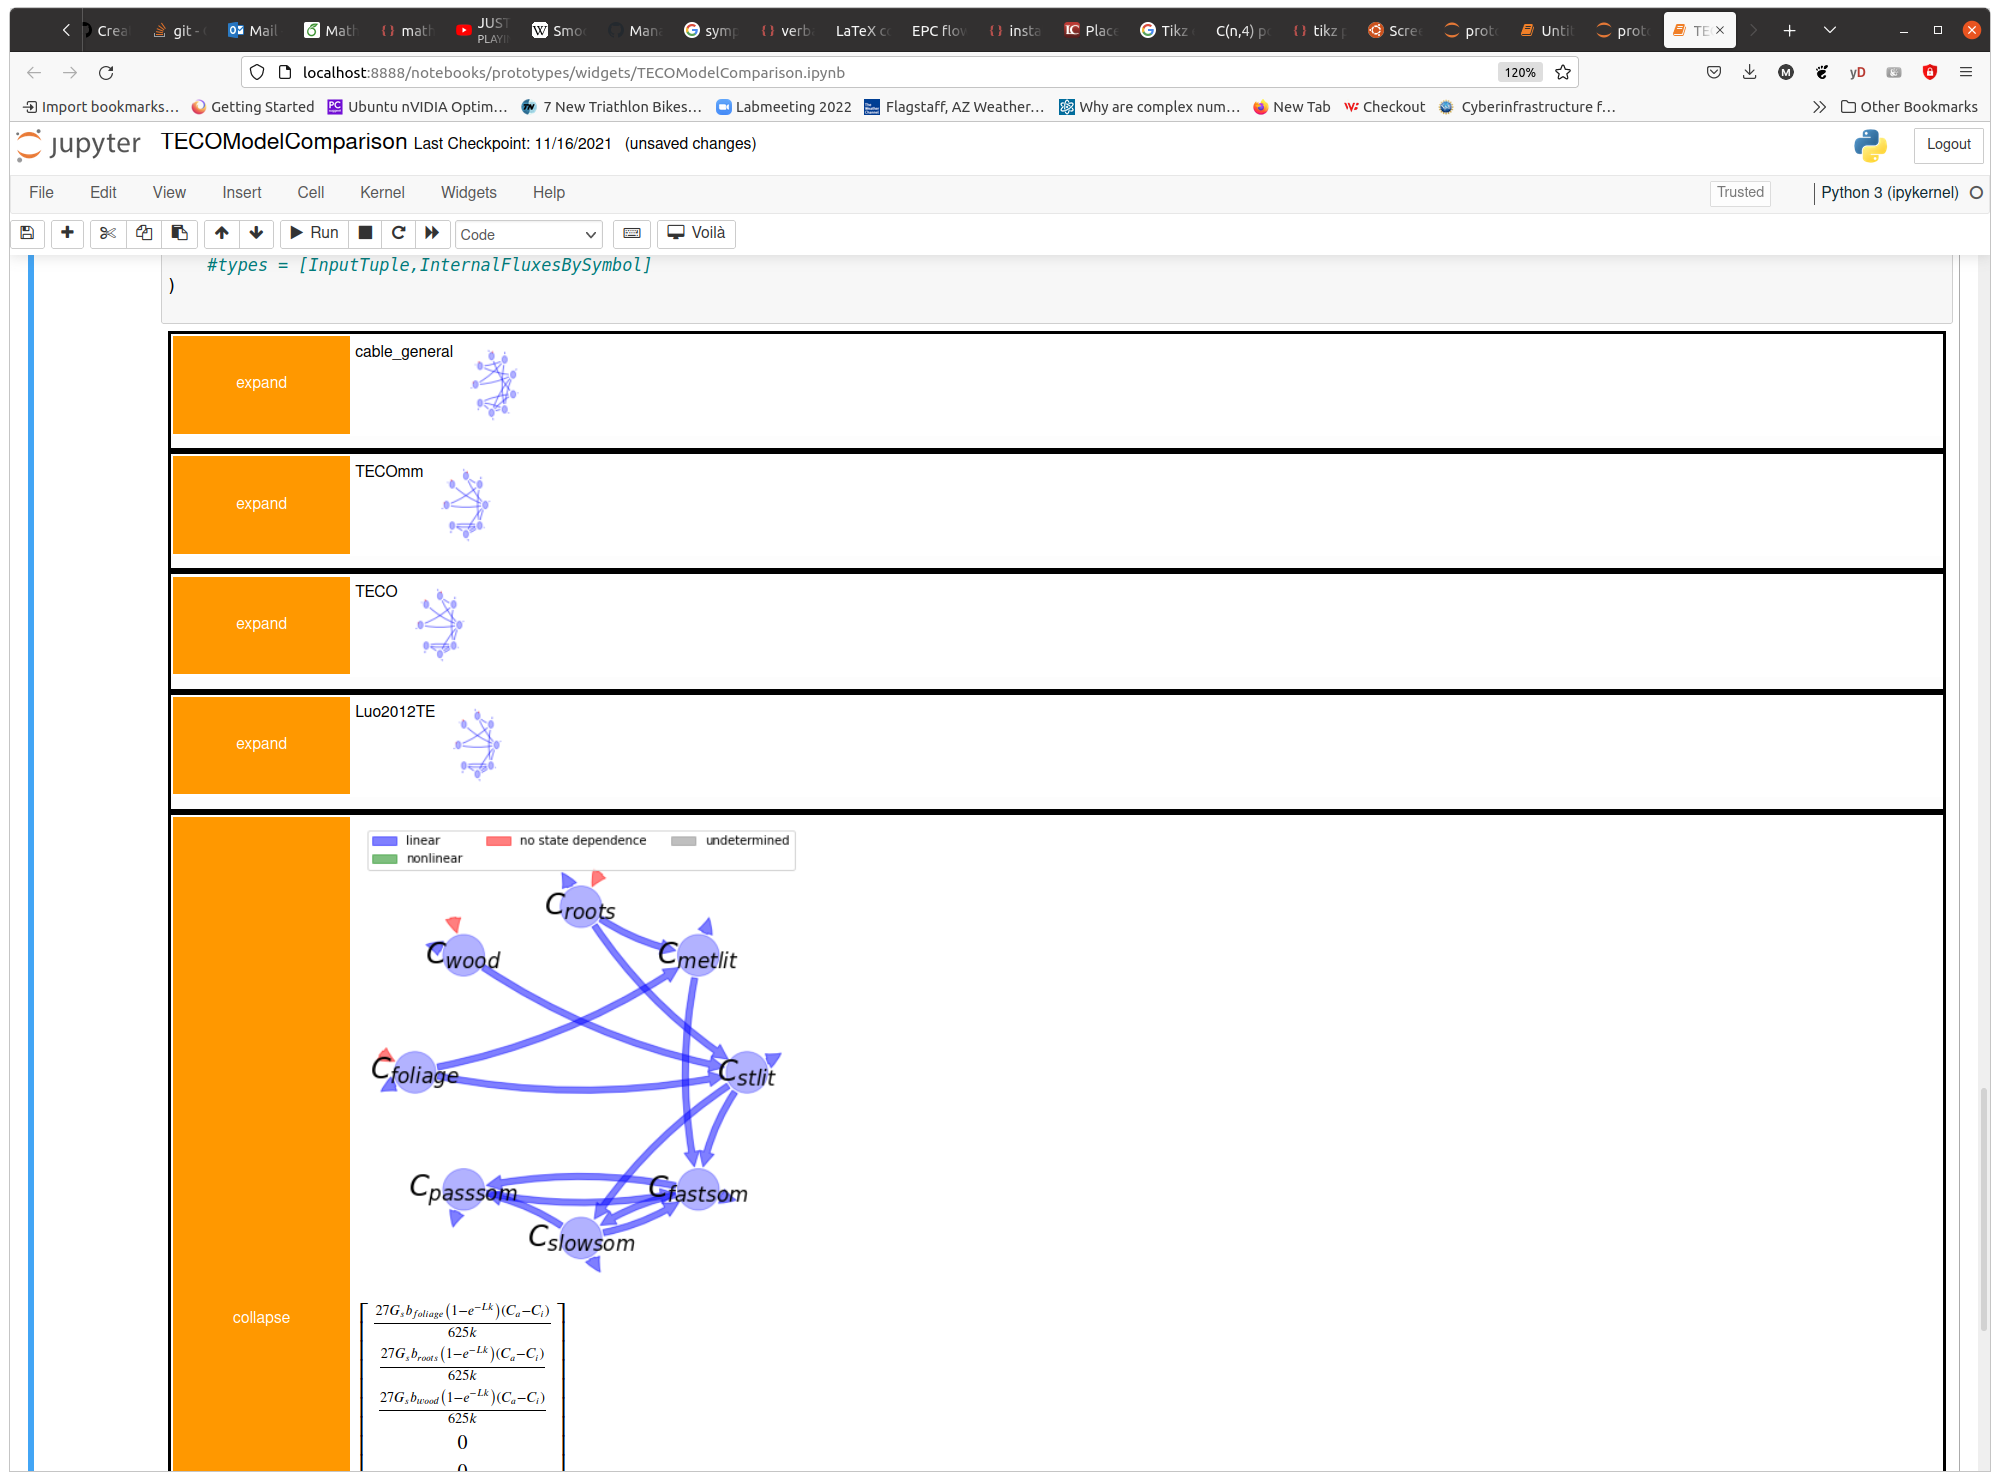
\includegraphics[width=.245\columnwidth]{ModelTable.png}
\end{center}
}

%----
%----

%%%%%%%%%%%%%%%%%%%%%%%%%%%%%%%%%%%%%%%%%%%%%%%%%%%%%%%%%%%%%%%%%%%%%%%%%%%%%%%%%%%----
\posterbox[adjusted title=Open Source Code and Data]{
  name=internalStructure,
  %column*=4,
  column=4,
  %sequence=3 between title and bottom then 4 between top and record
  below=title,
  %column=2,
  %span=1.5,
  %above=bottom
  }{
  
%\frametitle{Internal Structure of \texttt{bgc\_md2}}
%\begin{tikzpicture}[sibling distance=12em,
\section*{Internal Structure} 

\begin{tikzpicture}[sibling distance=28em,
  every node/.style = {shape=rectangle, rounded corners,
    draw, align=center,
    top color=white, bottom color=blue!20}]]
  \tikzstyle{level 1}=[sibling distance=20em]
  \tikzstyle{level 2}=[sibling distance=5em]
  \tikzstyle{level 3}=[sibling distance=3em]
  \tikzstyle{level 4}=[sibling distance=1.75em]
    \node {% <- this 'right of' is inherited; how to avoid?
    \begin{tikzpicture}[anchor=center]
      \node {\texttt{bgc\_md2}
      %\draw (0,0) -- (0,1);
      %\node[fill] at (0,.5) {};
      } 
      child{ node {models}
	 child{ node{rothC}
	    child{node {Fluxes}}
	    child{node {Pools}}
	    child{node {\dots}}
	}
      	child{ node {Wang}
	%    child{node {Fluxes}}
	%    child{node {Pools}}
	%    child{node {\dots}}
	}
      	child{ node {\dots}}
      }
      child{ node {computers}
	 child{node {Matrix(Fluxes)}}
	 %child{node {Fluxes(Matrix,Pools)}}
	 child{node {\dots}}
      };
    \end{tikzpicture}
    };
\end{tikzpicture}
  \begin{enumerate}
    \item
    \texttt{bgc\_md2} is not just a collection of models, described as sets of varible of special type like fluxes or matrice, but also 
    a collection of functions whose arguments and return values have these types.
    These functions are here called \texttt{computers} and use python type annotations.
    The computability graph used in the user interface and queries is derived from the 
    annotations of a set of functions.
    The set of properties (defined by the types) is growing as well as the functions connecting them.
  \end{enumerate}
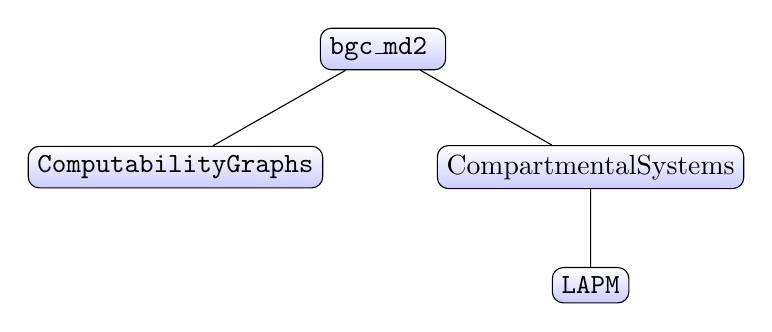
\begin{tikzpicture}[sibling distance=15em,
  every node/.style = {shape=rectangle, rounded corners,
    draw, align=center,
    top color=white, bottom color=blue!20}]]
    \node {
    	\texttt{bgc\_md2}
    }
    child { node {\texttt{ComputabilityGraphs}} }
	child { node[sibling distance=5em]{CompartmentalSystems}
	child { node (LAPM){\texttt{LAPM}} }
	%child [level distance=10em]{ node [style ={top color=white,bottom color=black!10}](SymPy){\texttt{SymPy}} }
	%child [level distance=10em]{ node [style ={top color=white,bottom color=black!10}](SymPy){\texttt{nupy}} }
   };
	%\draw[->] (LAPM) -- (SymPy); 
\end{tikzpicture}
  \begin{enumerate}
    \item
    The graph computation is outsourced into our package \texttt{ComputabilityGraphs} 
    \item
	    Many of the advanced diagnostic variables (age and transittime distributions) are computed using our other packages \texttt{LAPM} and \texttt{CompartmentalSystems} for which \texttt{bgc\_md2} acts as interface.
  \end{enumerate}
  \subsection*{Database records are python modules}
  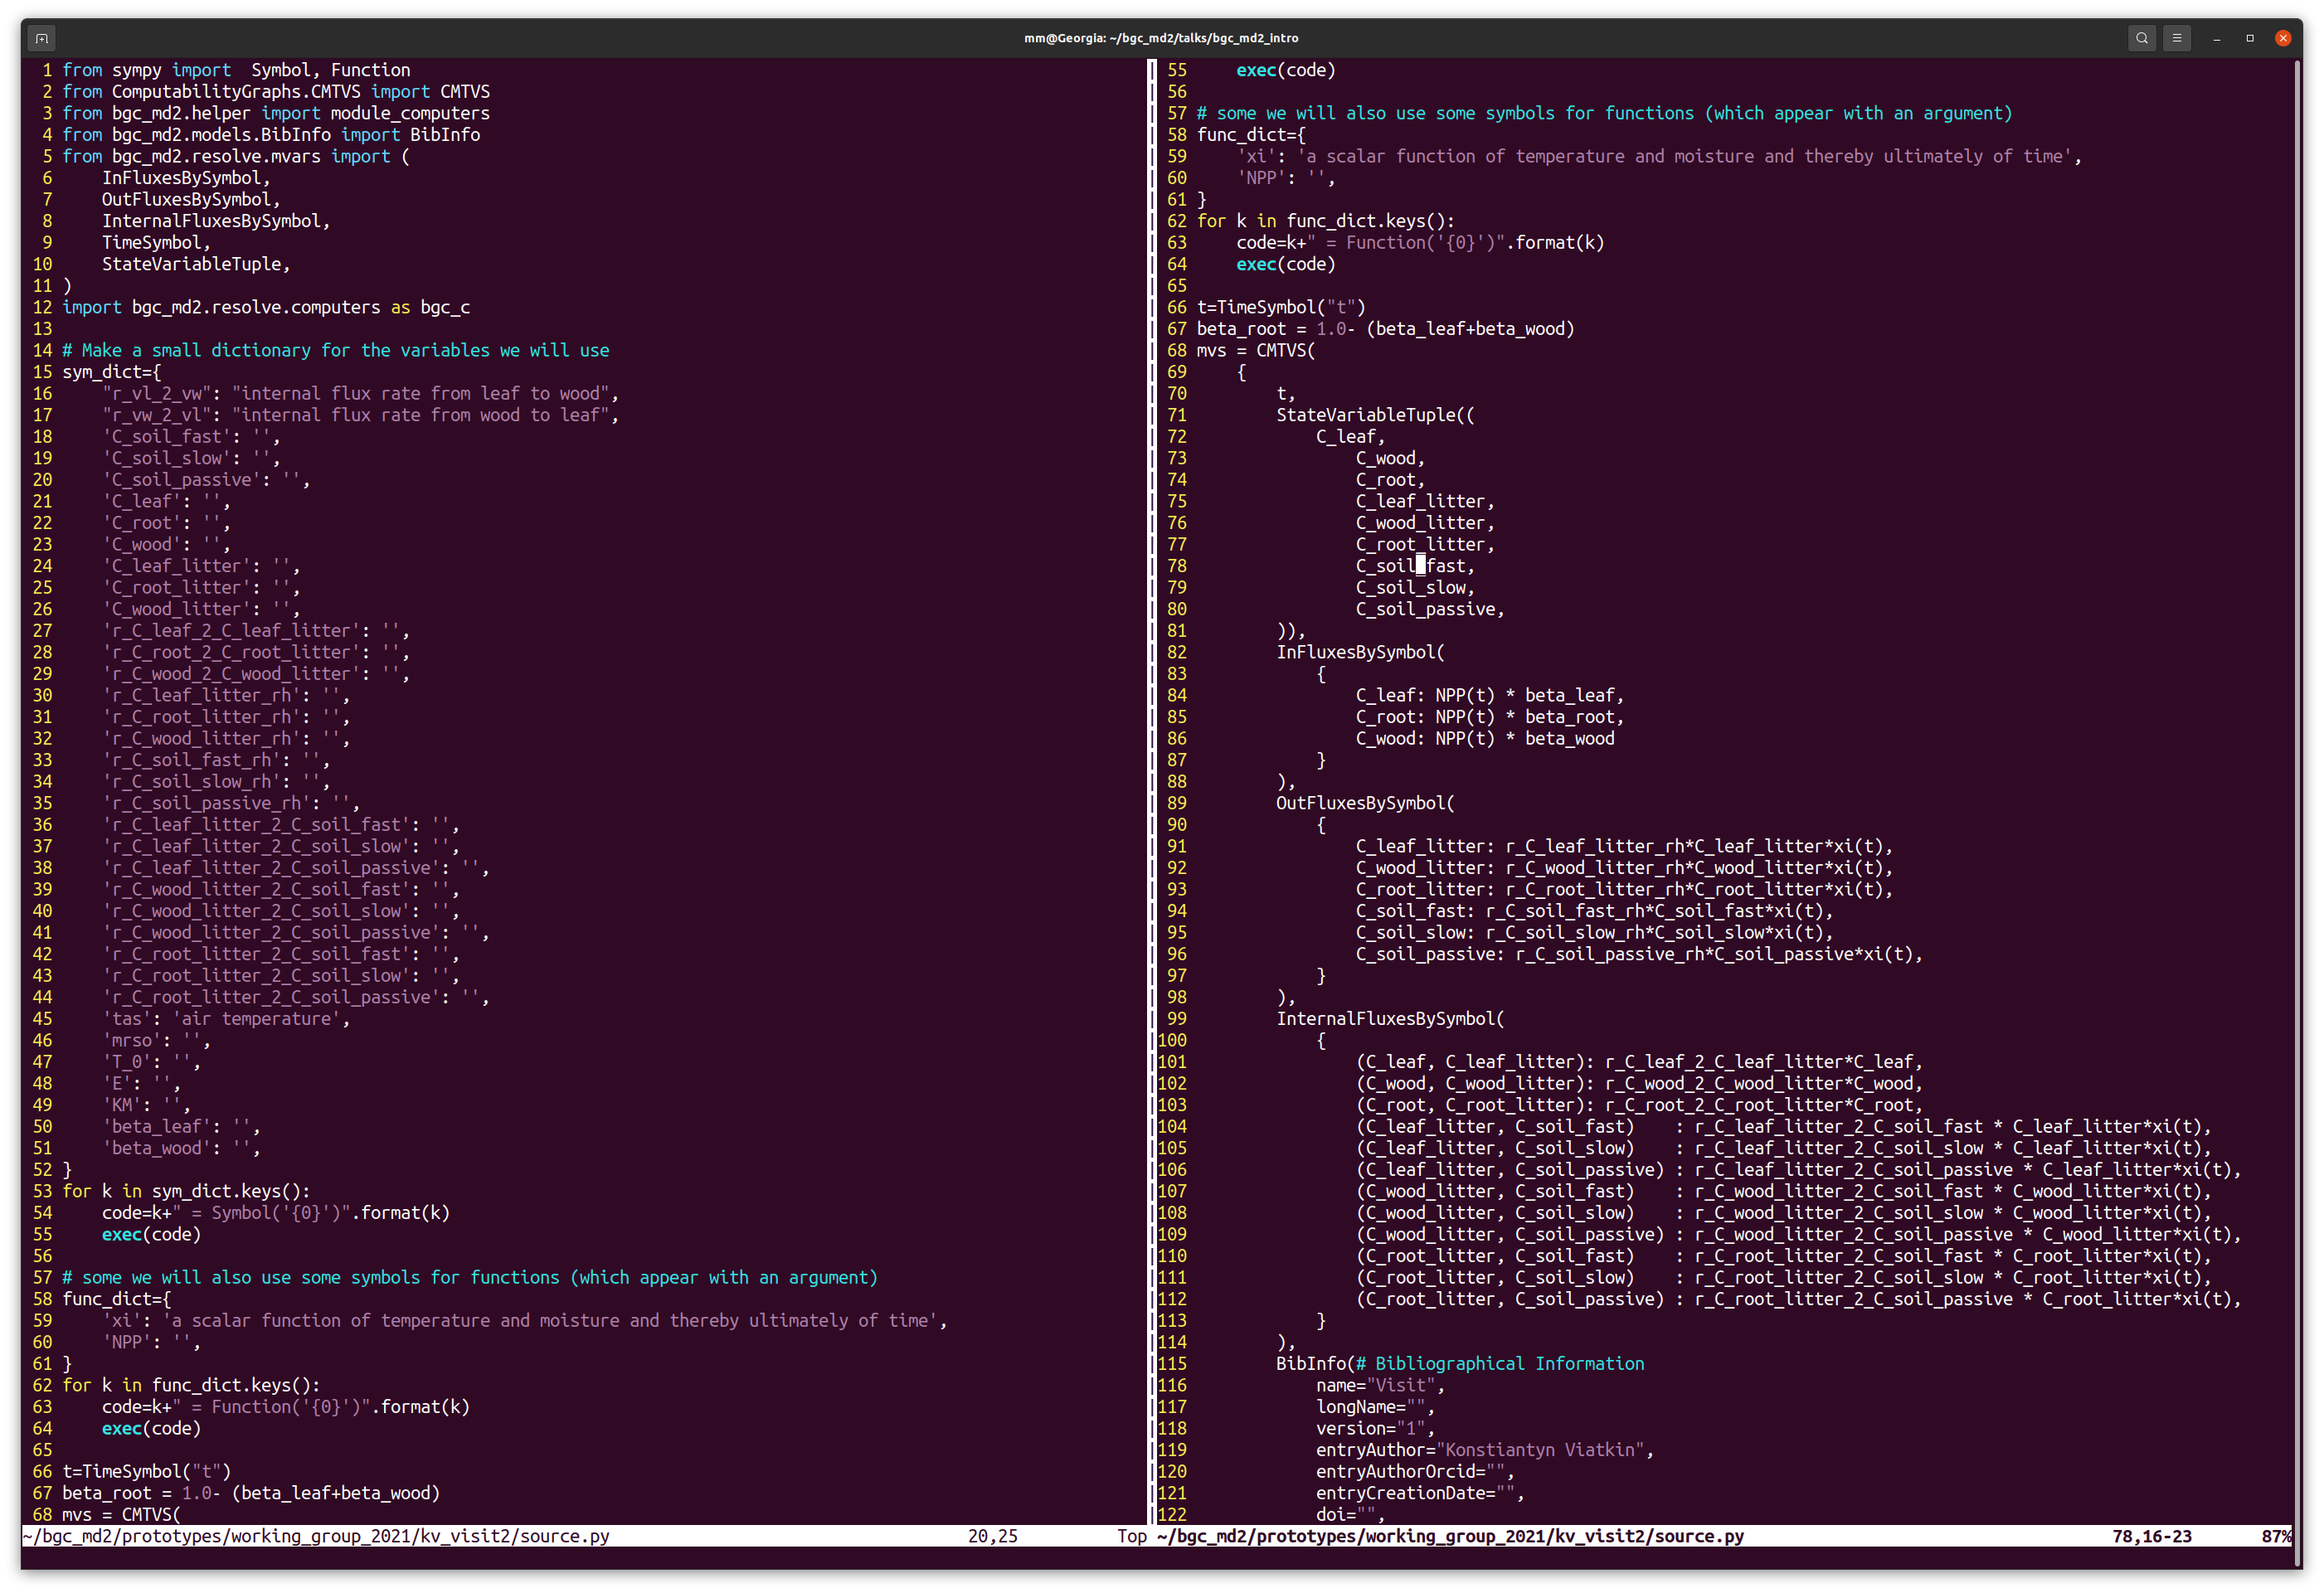
\includegraphics[width=\columnwidth]{source.py.png}
  \begin{enumerate}
    \item
    The picture shows the screen shot of the source code of the above model using sympy and some datatypes provided by \texttt{bgc\_md2}  .
    \item
    The entries of the database dont even have to be complete models. They are implemented in normal python and 
    have in common that they define a set of model properties and a set of functions to connect them.
    There is no special format necessary. 
    The creation of the symbolic formulation can be automated by all means available in python.
    Extra information can but does not have to be provided.
  \end{enumerate}
}
%%%%%%%%%%%%%%%%%%%%%%%%%%%%%%%%%%%%%%%%%%%%%%%%%%%%%%%%%%%%%%%%%%%%%%%%%%%%%%%%%%%%----
\posterbox[adjusted title=References]{
  name=references,
  %column*=4,
  column=4,
  below=internalStructure,
  %column=2,
  %span=1.5,
  %above=bottom
  }{
  \nocite{Luo2017Biogeosciences}
  \nocite{Rasmussen2016JMB}
  \nocite{Metzler2018PNAS}
	%\begin{thebibliography}{}
	%\bibitem[Metzler, Müller, Sierra, 2018]{Metzler2018PNAS}
	%Metzler, H., M{\"u}ller, M., and Sierra, C. (2018).
	%\newblock Transit-time and age distributions for nonlinear time-dependent
	%  compartmental systems.
	%\newblock {\em Proceedings of the National Academy of Sciences}, 115:201705296.
	%\end{thebibliography}
  \bibliographystyle{abbrvnat}
  \bibliography{TEE-clean.bib}
}
%%%%%%%%%%%%%%%%%%%%%%%%%%%%%%%%%%%%%%%%%%%%%%%%%%%%%%%%%%%%%%%%%%%%%%%%%%%%%%%%%%%%----
\posterbox[adjusted title=Contact]
    {
    name=contact,
    %column*=4,
    column=4,
    above=bottom}{
    blablalllllllllllllllllllllllllllll
}
\end{tcbposter}
\end{document}

